\documentclass[9pt]{beamer}

\usepackage{fancyvrb}


\usetheme[progressbar=frametitle]{metropolis}
\usepackage{appendixnumberbeamer}

\usepackage{booktabs}
\usepackage[scale=2]{ccicons}

\usepackage{pgfplots}
\usepgfplotslibrary{dateplot}

\usepackage{graphicx}
\usepackage{caption}
\usepackage{subcaption}
\usepackage{amssymb}
\usepackage{graphicx}
\usepackage{caption}
\usepackage{subcaption}
\usepackage{amsmath}
\usepackage{mathtools}
\usepackage{xspace}
\newcommand{\themename}{\textbf{\textsc{metropolis}}\xspace}



\usepackage[linesnumbered, ruled]{algorithm2e}
% \usepackage{algorithmic}
%%% optional fonts and color configuration
\SetAlFnt{\sffamily}
\renewcommand\ArgSty{\normalfont\sffamily}
\renewcommand\KwSty[1]{\textnormal{\textbf{\sffamily#1}}\unskip}
\SetAlCapFnt{\normalfont\sffamily\large}
\renewcommand\AlCapNameFnt{\sffamily\large}

%%% vertical rules in cyan color
\makeatletter
\renewcommand{\algocf@Vline}[1]{%     no vskip in between boxes but a strut to separate them, 
  \strut\par\nointerlineskip% then interblock space stay the same whatever is inside it
  \algocf@push{\skiprule}%        move to the right before the vertical rule
  \hbox{\bgroup\color{black}\vrule\egroup%
    \vtop{\algocf@push{\skiptext}%move the right after the rule
      \vtop{\algocf@addskiptotal #1}\bgroup\color{black}\Hlne\egroup}}\vskip\skiphlne% inside the block
  \algocf@pop{\skiprule}%\algocf@subskiptotal% restore indentation
  \nointerlineskip}% no vskip after
%
\renewcommand{\algocf@Vsline}[1]{%    no vskip in between boxes but a strut to separate them, 
  \strut\par\nointerlineskip% then interblock space stay the same whatever is inside it
  \algocf@bblockcode%
  \algocf@push{\skiprule}%        move to the right before the vertical rule
  \hbox{\bgroup\color{black}\vrule\egroup%               the vertical rule
    \vtop{\algocf@push{\skiptext}%move the right after the rule
      \vtop{\algocf@addskiptotal #1}}}% inside the block
  \algocf@pop{\skiprule}% restore indentation
  \algocf@eblockcode%
}
%
\makeatother
%%% end of optional fonts and color configuration

\SetKwProg{Fn}{Function}{}{}



\title{Complex Network Analysis \\
with Edge Uncertainty}
% \subtitle{Shortest Path and Centrality Measures}
\date{\textbf{Supervisor: Osmar R. Za\"{\i}ane}}
\author{\textbf{Chi Zhang}}
\institute{March 10, 2018}
% \titlegraphic{\hfill\includegraphics[height=1.5cm]{logo.pdf}}


\begin{document}
\setbeamercolor{background canvas}{bg=white}
\maketitle

\begin{frame}{Overview}
  \setbeamertemplate{section in toc}[sections numbered]
  \vspace{0.1in}
  \tableofcontents
\end{frame}

\section{Link Prediction}

\begin{frame}{Link Prediction - Problem Definition}
\begin{figure}
\centering
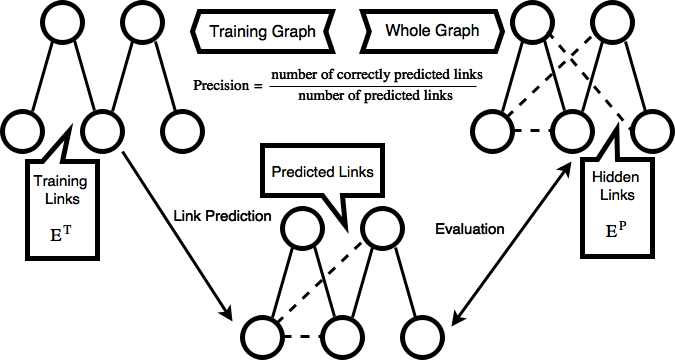
\includegraphics[scale = 0.4]{evaluation.png}
\caption{Evaluation procedures: Hidden true links are compared to predicted links. How many predicted links where truly there?}
\label{example}
\end{figure}
\end{frame}


\begin{frame}
\frametitle{Link Prediction - Previous Work - Similarity Metrics}
\textbf{Basic Ideas:} Two nodes, $\mathcal{V}_x$ and $\mathcal{V}_y$, are more likely to form a link if they have many common neighbors. 
\begin{itemize}
\item \textbf{Common Neighbors (CN)}: The simplest measure of the neighborhood overlap is the directed count:
\begin{equation}
s_{xy}=|\Gamma(x)\cap\Gamma(y)|
\end{equation}
Where $\Gamma(x)$ is the set of neighbors of node $\mathcal{V}_x$. 
\item \textbf{Resource Allocation (RA)}: The node $\mathcal{V}_x$ can send some resource to $\mathcal{V}_y$, with their common neighbors playing the role of transmitters. We assume that each transmitter has a unit of resource, and will evenly distribute to all its neighbors. As a results the amount of resource $\mathcal{V}_y$ received is defined as the similarity
between $\mathcal{V}_x$ and $\mathcal{V}_y$, which is:
\begin{equation}
s_{xy}=\sum_{z\in \Gamma(x)\cap\Gamma(y)}\frac{1}{k(z)}
\end{equation}
where $k(z)$ is the degree of node $\mathcal{V}_z$, namely $k(z) = |\Gamma(z)|$
\end{itemize}
\end{frame}

\begin{frame}
\frametitle{Link Prediction - Previous Work - Similarity Metrics for Weighted Graphs}
CN: $s_{xy}=|\Gamma(x)\cap\Gamma(y)|$

\textbf{Weighted Common Neighbors (WCN)}
\begin{equation}
s_{xy}=\sum_{z\in \Gamma(x)\cap\Gamma(y)}w(x,z)+w(y,z)
\end{equation}

RA: $s_{xy}=\sum_{z\in \Gamma(x)\cap\Gamma(y)}\frac{1}{k(z)}$

\textbf{Weighted Resource Allocation (WRA)}
\begin{equation}
s_{xy}=\sum_{z\in \Gamma(x)\cap\Gamma(y)}\frac{w(x,z)+w(y,z)}{s(z)}
\end{equation}

Here, $w(x, y) = w(y, x)$ denotes the weight of the link between nodes $\mathcal{V}_x$ and $\mathcal{V}_y$, and $s(x)=\sum_{z\in\Gamma(x)}w(x,z)$ is the strength of node $\mathcal{V}_x$.
\end{frame}

\begin{frame}{Link Prediction - Review of Previous Method}
  \begin{columns}[T,onlytextwidth]
    \column{0.4\textwidth}
      \begin{figure}
      \centering
      
      \begin{subfigure}[b]{\textwidth}
         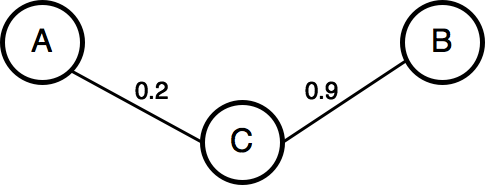
\includegraphics[scale = 0.25]{common_neighbor_2.png}
      \end{subfigure}

      \begin{subfigure}[b]{\textwidth}
         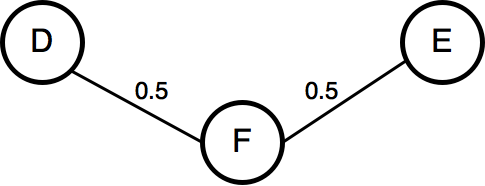
\includegraphics[scale = 0.25]{common_neighbor_1.png}
      \end{subfigure}

      \caption{An example showing the problem when considering the probability as a weight. A-B would seem to have a higher probability to exist than D-E}
      \label{example}
      \end{figure}

    \column{0.5\textwidth}
    \textbf{Weighted Common Neighbors (WCN)}
    \begin{align*}
    s_{xy}=\sum_{z\in \Gamma(x)\cap\Gamma(y)}w(x,z)+w(y,z)
    \end{align*}
      \begin{align*}
      s_{AB} =0.2 + 0.9 = 1.1
      \end{align*}
      \begin{align*}
      s_{DE} =0.5 + 0.5 = 1.0 < 1.1
      \end{align*}
      \newline
      \newline
	Nodes $\mathcal{V}_A$ and $\mathcal{V}_B$ are more likely to be connected than nodes $\mathcal{V}_D$ and $\mathcal{V}_E$.
  \end{columns}
\end{frame}

\begin{frame}{Link Prediction - Review of Previous Method}
\begin{figure}
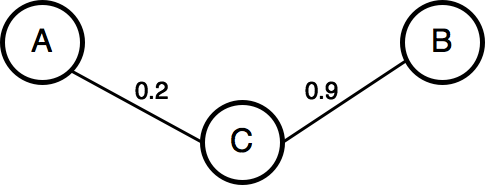
\includegraphics[scale = 0.2]{common_neighbor_2.png}
\hspace{1cm}
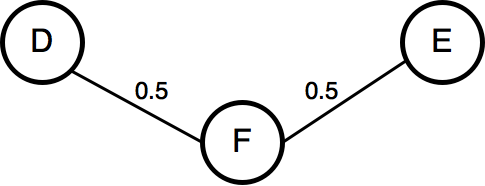
\includegraphics[scale = 0.2]{common_neighbor_1.png}
\centering
% \caption{An example showing the problem when considering the probability as a weight. A-B would seem to have a higher probability to exist than D-E}
% \label{example}
\end{figure}

\begin{figure}
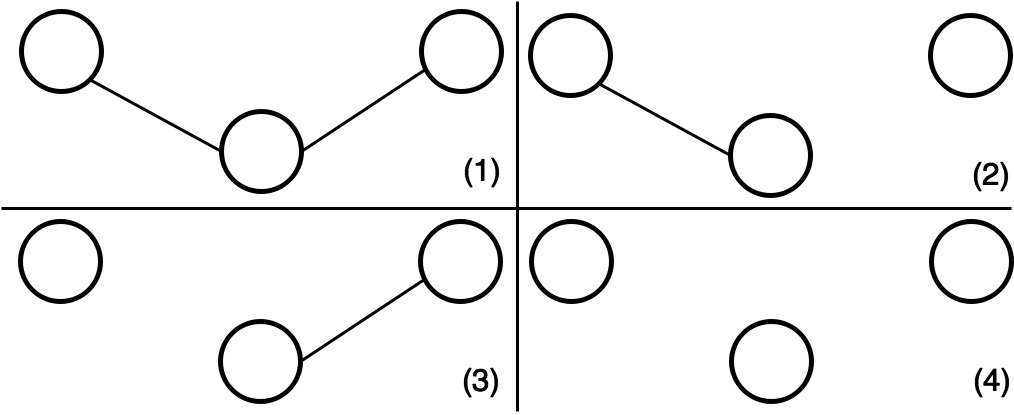
\includegraphics[scale = 0.18]{possible_world.png}
\centering
\caption{Possible worlds for two uncertain links between three nodes}
\label{example}
\end{figure}

Given an uncertain network $\mathcal{G = (V,E,P)}$, we can sample each edge in $\mathcal{G}$ according to the probability $\mathcal{P}(e)$ to generate the possible graph $G = (V_G,E_G)$. We have $E_G \in \mathcal{E}$ and $V_G \in \mathcal{V}$.
\begin{equation}
Pr(G) = \prod_{e\in E_G}\mathcal{P}(e)\prod_{e\in \mathcal{E}, e\notin E_G}(1-\mathcal{P}(e))
\end{equation}

\end{frame}

\begin{frame}{Link Prediction - Review of Previous Method}
\begin{figure}
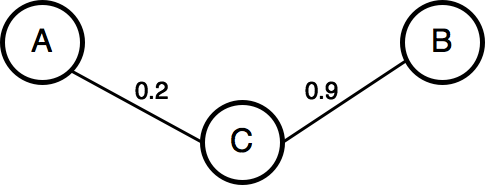
\includegraphics[scale = 0.23]{common_neighbor_2.png}
\hspace{1cm}
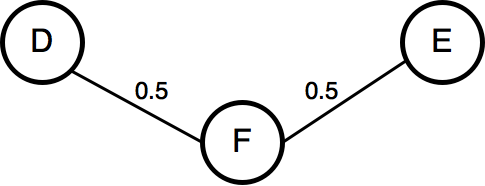
\includegraphics[scale = 0.23]{common_neighbor_1.png}
\centering
% \caption{An example showing the problem when considering the probability as a weight. A-B would seem to have a higher probability to exist than D-E}
% \label{example}
\end{figure}
\begin{align*}
Pr(G) = \prod_{e\in E_G}\mathcal{P}(e)\prod_{e\in \mathcal{E}, e\notin E_G}(1-\mathcal{P}(e))
\end{align*}
\begin{align*}
\text{CN: }s_{xy}=|\Gamma(x)\cap\Gamma(y)|
\end{align*}

$s_{AB}=1 \Rightarrow P=0.2\times 0.9=0.18$ 

$s_{AB}=0 \Rightarrow P=0.2\times(1-0.9)+(1-0.2)\times0.9+(1-0.2)\times(1-0.9)=0.82$

$s_{DE}=1 \Rightarrow P=0.5\times 0.5=0.25$ 

$s_{DE}=0 \Rightarrow P=0.5\times(1-0.5)+(1-0.5)\times0.5+(1-0.5)\times(1-0.5)=0.75$

The probability of $s_{DE}=1$ is larger than the probability of $s_{AB}=1$. 
\end{frame}


\begin{frame}{Link Prediction - Neighbor-based Metrics for Uncertain Graphs}

\textbf{Uncertain Common Neighbors (UCN)}
\begin{equation}
s_{xy}=\sum_{G\in \mathcal{G}}( Pr(G)\times|\Gamma_G(x)\cap\Gamma_G(y)|)
\end{equation}
% \begin{equation}
% s_{xy}=\sum_{z\in \Gamma(x)\cap\Gamma(y)}p(x,z)\times p(y,z)
% \end{equation}

\textbf{Uncertain Resource Allocation (URA)}
\begin{equation}
s_{xy}=\sum_{G\in \mathcal{G}}( Pr(G)\times\sum_{z\in \Gamma_G(x)\cap\Gamma_G(y)}\frac{1}{k_G(z)})
\end{equation}

\end{frame}

\begin{frame}{Link Prediction - UCN Complexity Analysis}
\begin{align*}
s_{xy}&=\sum_{G\in \mathcal{G}}( Pr(G)\times|\Gamma_G(x)\cap\Gamma_G(y)|) \textcolor{red}{\text{$\Rightarrow O(2^{|\mathcal{E}|}k)$}}\\
&=\sum_{G\in \mathcal{G}}Pr(G)\sum_{z\in \Gamma(x)\cap\Gamma(y)}\mathbb{I}_{\Gamma_G(x)\cap\Gamma_G(y)}(z)\\
&=\sum_{z\in \Gamma(x)\cap\Gamma(y)}\sum_{G\in \mathcal{G}}Pr(G)\times\mathbb{I}_{\Gamma_G(x)\cap\Gamma_G(y)}(z)\\
&=\sum_{z\in \Gamma(x)\cap\Gamma(y)}\mathcal{P}_{x,z}\times\mathcal{P}_{y,z} \textcolor{red}{\text{$\Rightarrow O(K)$}}
\end{align*}

When $z\in \Gamma_G(x)\cap\Gamma_G(y)$, $\mathbb{I}_{\Gamma_G(x)\cap\Gamma_G(y)}(z)=1$. In other cases, $\mathbb{I}_{\Gamma_G(x)\cap\Gamma_G(y)}(z)=0$.

$k$ is nodes' average degree in the possible world.

$K$ is the nodes' average degree in the uncertain network.
\end{frame}


\begin{frame}{Link Prediction - URA Complexity Analysis}
\begin{align*}
s_{xy}&=\sum_{G\in \mathcal{G}}( Pr(G)\times\sum_{z\in \Gamma_G(x)\cap\Gamma_G(y)}\frac{1}{k_G(z)}) \textcolor{red}{\text{$\Rightarrow O(2^{|\mathcal{E}|}k)$}}\\
&=\sum_{z\in \Gamma(x)\cap\Gamma(y)}\sum_{G\in \mathcal{G}}Pr(G)\times\mathbb{I}_{\Gamma_G(x)\cap\Gamma_G(y)}(z)\times \frac{1}{k_G(z)}\\
&=\sum_{z\in \Gamma(x)\cap\Gamma(y)}\sum_{{G_z}\in \mathcal{G}_z}Pr({G_z})\times\mathbb{I}_{\Gamma_{G_z}(x)\cap\Gamma_{G_z}(y)}(z)\times \frac{1}{k_{G_z}(z)}\textcolor{red}{\text{$\Rightarrow O(2^{K}t)$}}\\
\end{align*}
$\mathcal{G}_z$ here stands for the uncertain sub-graph formed by edges connecting to node $\mathcal{V}_z$, and $G_z$ is the possible world based on the uncertain sub-graph $\mathcal{G}_z$.

When $z\in \Gamma_G(x)\cap\Gamma_G(y)$, $\mathbb{I}_{\Gamma_G(x)\cap\Gamma_G(y)}(z)=1$. In other cases, $\mathbb{I}_{\Gamma_G(x)\cap\Gamma_G(y)}(z)=0$.

$k$ is nodes' average degree in the possible world.

$K$ is the nodes' average degree in the uncertain network.

$t=|\Gamma_G(x)\cap\Gamma_G(y)|$
\end{frame}

\begin{frame}{Link Prediction - An Efficient Algorithm for the Calculation of URA}

Only when both edges $\mathcal{E}_{xz}$ and $\mathcal{E}_{yz}$ exist, node $\mathcal{V}_z$ is the common neighbor of $\mathcal{V}_x$ and $\mathcal{V}_y$ in the possible world $G$. Assume node $\mathcal{V}_z$ has $m$ extra edges in an uncertain graph except edges $\mathcal{E}_{xz}$ and $\mathcal{E}_{yz}$. We have two ways to calculate $s_{xy}$:

(1) Iterate through all possible worlds, calculate each possible world's possibility and its corresponding count of edges.

(2) Iterate through all the possible number of edges and calculate their corresponding probability.

\begin{align*}
s_{xy}&=\sum_{z\in \Gamma(x)\cap\Gamma(y)}\sum_{{G_z}\in \mathcal{G}_z}Pr({G_z})\times\mathbb{I}_{\Gamma_{G_z}(x)\cap\Gamma_{G_z}(y)}(z)\times \frac{1}{k_{G_z}(z)}\\
&=\sum_{z\in \Gamma(x)\cap\Gamma(y)}\mathcal{P}_{x,z}\times\mathcal{P}_{y,z} \times \sum_{n=0}^{m}(P_{1\rightarrow m}^n \times \frac{1}{n+2})
\end{align*}

We can index the $m$ edges connecting to $\mathcal{V}_z$ from 1 to $m$. $P_{1\rightarrow m}^n$ here stands for from edges $e_1$ to $e_m$, the probability that exactly $n$ among them exist in possible worlds.

\end{frame}


\begin{frame}{Link Prediction - An Efficient Algorithm for the Calculation of URA}

\begin{align*}
s_{xy}=\sum_{z\in \Gamma(x)\cap\Gamma(y)}\mathcal{P}_{x,z}\times\mathcal{P}_{y,z} \times \sum_{n=0}^{m}(P_{1\rightarrow m}^n \times \frac{1}{n+2})
\end{align*}

We need to compute $P_{1\rightarrow m}^0, P_{1\rightarrow m}^1, ..., P_{1\rightarrow m}^m$.

A divide and conquer algorithm:

1) Divide the probability list into $n$ sublists, each containing 1 element, and compute the probability of having and not having this item respectively.

2) Repeatedly merge sublists to compute probabilities for sublists with more than 1 element. The the equation for merging the left half sublist and the right half sublist.

\begin{equation}
P_{1\rightarrow m}^n=\sum_{i=max(0,n-\lceil m/2 \rceil)}^{min(n,\lfloor m/2 \rfloor)}P_{1\rightarrow{\lfloor m/2 \rfloor}}^i P_{{\lfloor m/2 \rfloor}+1\rightarrow m}^{n-i}
\end{equation}

\end{frame}

\begin{frame}{Link Prediction - An Efficient Algorithm for the Calculation of URA}

\begin{algorithm}[H]
% https://tex.stackexchange.com/questions/26566/reduce-pseudocode-font-size-not-global
% \algsetup{linenosize=\tiny}
  \scriptsize
\KwData{Probability List $uncertainEdgeList$}
\KwResult{The probability list $probList$ of existing $n$ among $m$ edges, $n\in [0,m]$}
$uncertainEdgeListLength \leftarrow len(uncertainEdgeList)$\;
return $kEdge(0, uncertainEdgeListLength-1)$\;
// Inner Function\;
\Fn{kEdge(i, j)}{
 $length\leftarrow j-i+1$\;
 \eIf{$length=1$}{return $[1-uncertainEdgeList[i], uncertainEdgeList[i]]$}
 {
 $leftLength\leftarrow length // 2$\;
 $rightLength\leftarrow length - leftLength$\;
 // Divide Phase\;
 $left\leftarrow kEdge(i, i+leftLength-1)$\;
 $right \leftarrow kEdge(i+leftLength, j)$\;
 $probList \leftarrow [0] \times (length+1)$\;
 \For{each $n \in [0, length]$}{
	 \For{each $k \in [0, n]$}{
     	\If{$k<=leftLength$ and $n-k<=rightLength$}{
        	// Merge Phase\;
        	$probList[n] \leftarrow probList[n] + left[k]\times right[n-k]$\;
		}
 	}
 }
 return $probList$\;
 }
}
\caption{kEdgeProbability}
\end{algorithm}

\end{frame}


\begin{frame}{Link Prediction - An Efficient Algorithm for the Calculation of URA}


\begin{figure}
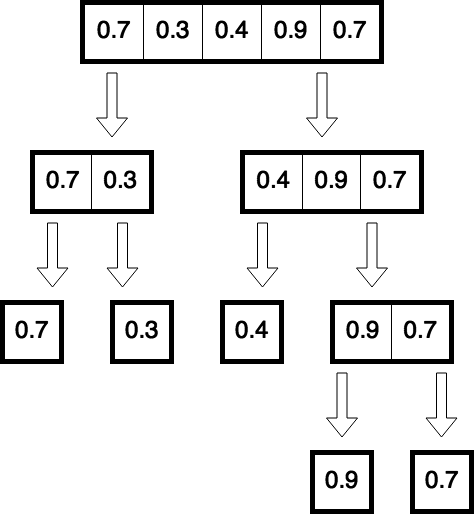
\includegraphics[scale = 0.35]{5_sample_divide.png}
\centering
\caption{Algorithm Example: Divide Phase}
\label{example}
\end{figure}


\end{frame}

\begin{frame}{Link Prediction - An Efficient Algorithm for the Calculation of URA}


\begin{figure}
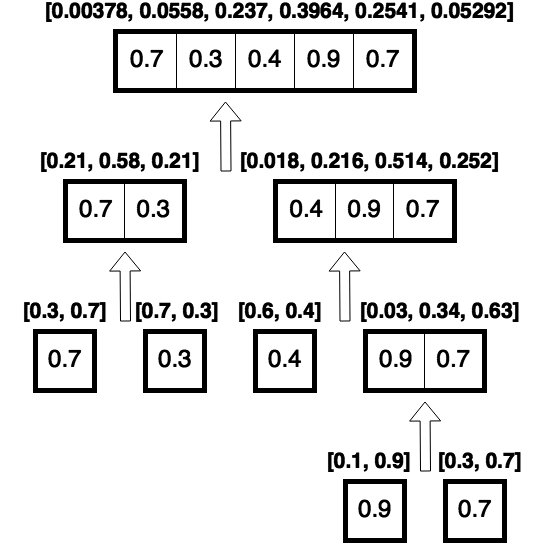
\includegraphics[scale = 0.35]{5_sample_conquer.png}
\centering
\caption{Algorithm Example: Merge Phase}
\label{example}
\end{figure}


\end{frame}


\begin{frame}{Link Prediction - An Efficient Algorithm for the Calculation of URA}
\begin{equation}
P_{1\rightarrow m}^n=\sum_{i=max(0,n+k-m)}^{min(n,k)}P_{1\rightarrow k}^i P_{k+1\rightarrow m}^{n-i}
\label{URA-equation}
\end{equation}

$A = [P_{1\rightarrow m+2}^0, P_{1\rightarrow m+2}^1, ..., P_{1\rightarrow m+2}^{m+2}]$

$B = [P_{1\rightarrow m}^0, P_{1\rightarrow m}^1, ..., P_{1\rightarrow m}^{m}]$

$C = [P_{m+1\rightarrow m+2}^0, P_{m+1\rightarrow m+2}^1, P_{m+1\rightarrow m+2}^2]$

\begin{align*}
\left\{
\begin{aligned}
P_{m+1\rightarrow m+2}^2 P_{1\rightarrow m}^{m} = P_{1\rightarrow m+2}^{m+2}\\
P_{m+1\rightarrow m+2}^1 P_{1\rightarrow m}^{m} + P_{m+1\rightarrow m+2}^2 P_{1\rightarrow m}^{m-1} = P_{1\rightarrow m+2}^{m+1}\\
P_{m+1\rightarrow m+2}^0 P_{1\rightarrow m}^{m} + P_{m+1\rightarrow m+2}^1 P_{1\rightarrow m}^{m-1} + P_{m+1\rightarrow m+2}^2 P_{1\rightarrow m}^{m-2} = P_{1\rightarrow m+2}^{m}\\
P_{m+1\rightarrow m+2}^0 P_{1\rightarrow m}^{m-1} + P_{m+1\rightarrow m+2}^1 P_{1\rightarrow m}^{m-2} + P_{m+1\rightarrow m+2}^2 P_{1\rightarrow m}^{m-3} = P_{1\rightarrow m+2}^{m-1}\\
...\\
P_{m+1\rightarrow m+2}^0 P_{1\rightarrow m}^{3} + P_{m+1\rightarrow m+2}^1 P_{1\rightarrow m}^{2} + P_{m+1\rightarrow m+2}^2 P_{1\rightarrow m}^{1} = P_{1\rightarrow m+2}^3\\
P_{m+1\rightarrow m+2}^0 P_{1\rightarrow m}^{2} + P_{m+1\rightarrow m+2}^1 P_{1\rightarrow m}^{1} + P_{m+1\rightarrow m+2}^2 P_{1\rightarrow m}^{0} = P_{1\rightarrow m+2}^2\\
\end{aligned}
\right.
\end{align*}
\end{frame}

\begin{frame}{Link Prediction - An Efficient Algorithm for the Calculation of URA}

\begin{algorithm}[H]
\KwData{An uncertain graph $\mathcal{G}$.}
\KwResult{Probability lists for all nodes in $\mathcal{G}$ saved in a hash table $dict$}
Hash table $dict \leftarrow \{\}$\;
\For{each node $\mathcal{V}_z \in \mathcal{G}$}{
Array $uncertainEdgeList \leftarrow$ all uncertain edges connecting to node $\mathcal{V}_z$\;
$dict[\mathcal{V}_z]\leftarrow kEdgeProbability(uncertainEdgeList)$\;
}
return $dict$\;
\caption{Initialization}
\end{algorithm}

\end{frame}


\begin{frame}{Link Prediction - An Efficient Algorithm for the Calculation of URA}

\begin{algorithm}[H]
  \scriptsize
\KwData{Nodes $\mathcal{V}_x$, $\mathcal{V}_y$, an uncertain graph $\mathcal{G}$ and the hash table $dict$ after running Algorithm 2}
\KwResult{Resource Allocation value for nodes $\mathcal{V}_x$ and $\mathcal{V}_y$ in $\mathcal{G}$}
$result \leftarrow 0$\;
\For{each node $\mathcal{V}_z \in \Gamma(x)\cap\Gamma(y)$}{
Array $uncertainEdgeList \leftarrow [ ]$\;
$probValue \leftarrow 1$\;
	\For{each node $\mathcal{V}_m$ connecting to node $\mathcal{V}_z$}{
    	\If{$\mathcal{V}_m=\mathcal{V}_x$ or $\mathcal{V}_m=\mathcal{V}_y$}{
        	$probValue \leftarrow probValue \times \mathcal{P}_{m,z}$\;
        	add $\mathcal{P}_{m,z}$ to $uncertainEdgeList$\;
        }
    }
    Array $probListC \leftarrow kEdgeProbability(uncertainEdgeList)$\;
    Array $probListA \leftarrow dict[\mathcal{V}_z]$\;
    Array $probListB \leftarrow $ use $probListA$ and $probListC$ to calculate $probListB$ based on the Equation (\ref{URA-equation})\;
    $oneNodeResult \leftarrow 0$\;
    \For{each $i \in [0,len(probListB))$}{
    	$oneNodeResult \leftarrow oneNodeResult + probListB[i] \times \frac{1}{i+2}$\;
    }
    $result \leftarrow result + probValue \times oneNodeResult$\;
}
return $result$\;
\caption{Resource Allocation Value Calculation}
\end{algorithm}

\end{frame}



\begin{frame}{Link Prediction - Experiment}
\begin{table}[H]
\centering
\caption{Algorithm List}
\label{algorithm-list-link}
\begin{tabular}{c|c}
\hline
Algorithm Name & Description                                                                                                                                                                       \\ \hline
CN/RA          & \begin{tabular}[c]{@{}c@{}}Pay no attention to probabilities\\  and use the original metrics.\end{tabular}                                                                        \\ \hline
WCN/WRA        & \begin{tabular}[c]{@{}c@{}}Regard probability as weight\\  and use weighted metrics.\end{tabular}                                                                                 \\ \hline
UCN/URA        & \begin{tabular}[c]{@{}c@{}}Use our uncertain version\\  of graph proximity measures.\end{tabular}                                                                                 \\ \hline
SRW2           & \begin{tabular}[c]{@{}c@{}}Pay no attention to probabilities and \\run local random walk algorithm, and we choose $t=2$\end{tabular}     \\ \hline
SRW3           & \begin{tabular}[c]{@{}c@{}}Pay no attention to probabilities and \\run local random walk algorithm, and we choose $t=3$\end{tabular}     \\ \hline
LNB-CN         & \begin{tabular}[c]{@{}c@{}}Pay no attention to probabilities and\\ use Local Na{\"\i}ve Bayes form of Common Neighbors\end{tabular}    \\ \hline
LNB-RA         & \begin{tabular}[c]{@{}c@{}}Pay no attention to probabilities and\\ use Local Na{\"\i}ve Bayes form of Resource Allocation\end{tabular} \\ \hline
\end{tabular}
\end{table}

\end{frame}


\begin{frame}{Link Prediction - Experiment}

\begin{table}[H]
\centering
\caption{Comparative Results for the original, weighted and uncertain versions of Common Neighbors and Resource Allocation}
\label{experiment-result-link}
\begin{tabular}{c|c|c|c|c|c|c}
\hline
Datasets   & CN      & WCN    & UCN               & RA       & WRA      & URA \\ \hline
PPI                       & 0.472   & 0.5045 & \textbf{0.5288} & 0.4123   & 0.45     & \textbf{0.5728}\\ \hline
Enron                     & 0.49    & 0.52   & \textbf{0.61}   & 0.51     & 0.47     & \textbf{0.52}\\ \hline
Synthetic Network         & 0.5812  & 0.5954 & \textbf{0.6043} & 0.6075   & 0.6124   & \textbf{0.6233}\\ \hline
\end{tabular}

\end{table}

\begin{table}[]
\centering
%\caption{My caption}
%\label{my-label}
\begin{tabular}{c|c|c|c|c}
\hline
Datasets          & SRW2 \cite{liu2010link}   & SRW3 \cite{liu2010link}  & LNB-CN \cite{liu2011link} & LNB-RA \cite{liu2011link} \\ \hline
PPI               & 0.4136 & 0.5284 & 0.4856 & 0.4992 \\ \hline
Enron             & 0.43   & 0.45   & 0.55   & 0.46   \\ \hline
Synthetic Network & 0.5852 & 0.5992 & 0.5962 & 0.5885 \\ \hline
\end{tabular}
\end{table}

\end{frame}


\begin{frame}{Link Prediction - Experiment}

\begin{figure}
\centering
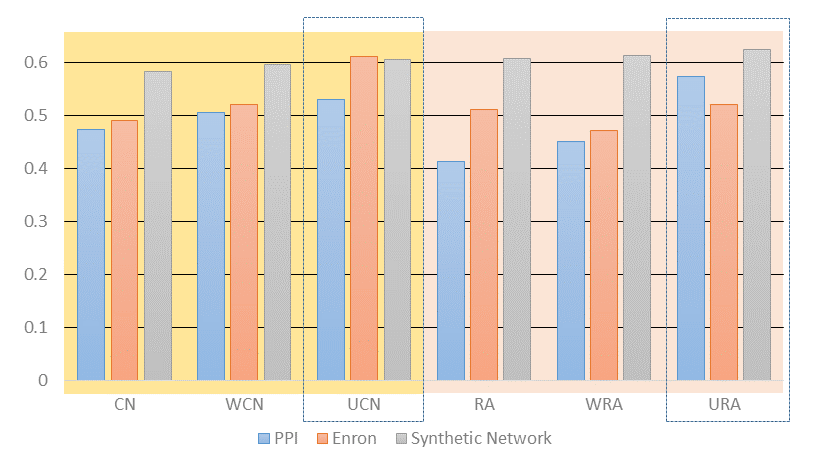
\includegraphics[scale = 0.9]{Result-Fig1.png}
\caption{Visual comparison of the accuracy for link prediction with UCN and URA with wighted and unweighted versions.}
\label{example}
\end{figure}

\end{frame}




\begin{frame}{Link Prediction - Experiment}

\begin{figure}
\centering
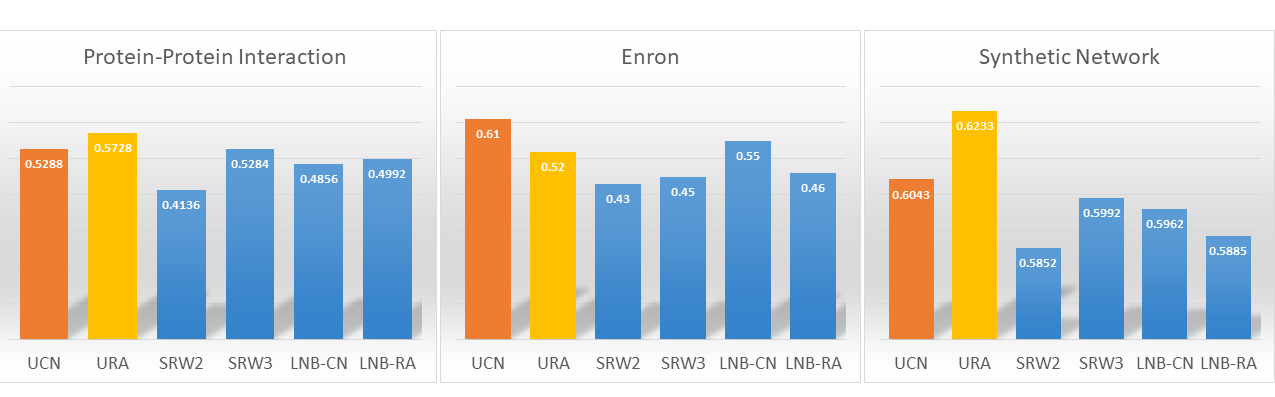
\includegraphics[scale = 0.6]{Results-Fig2.png}
\caption{Comparison of the accuracy for link prediction with UCN and URA against SRW \cite{liu2010link} and LNB \cite{liu2011link}.}
\label{example}
\end{figure}

\end{frame}

\section{Local Community Detection}


\begin{frame}{Local Community Detection - Definition}

\begin{figure}
\centering
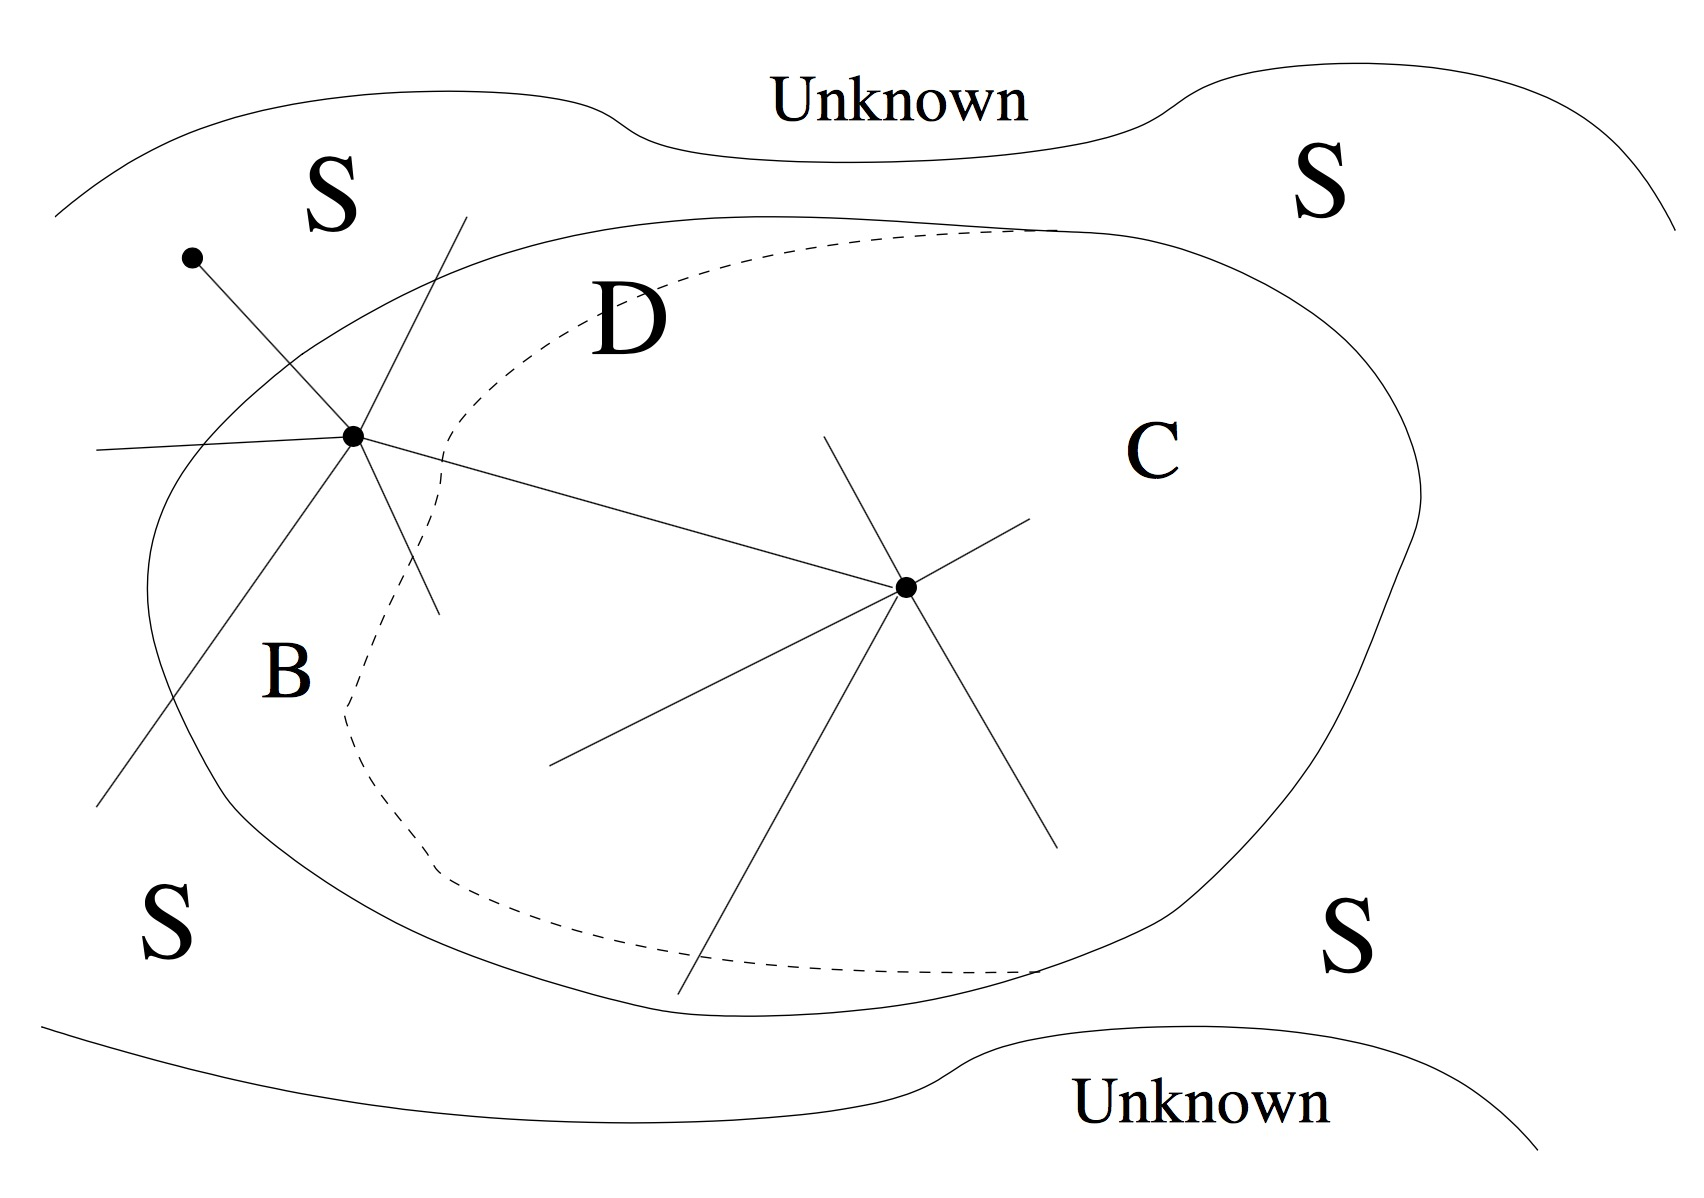
\includegraphics[scale = 0.1]{localCommunityDefinition.jpeg}
\caption{Local Community Definition}
\label{Local_Community_Definition}
\end{figure}
\small % https://tex.stackexchange.com/questions/24599/what-point-pt-font-size-are-large-etc

$\mathcal{D}$ denotes the known local community of the graph (for the start node). 

$\mathcal{S}$ contains nodes that are possible neighbors of nodes in $\mathcal{D}$ but do not belong to $\mathcal{D}$. 

Nodes in $\mathcal{D}$ can be split into two groups: the core node set $\mathcal{C}$, where any node $c_i\in \mathcal{C}$ has no outward links, which means all possible neighbors of $c_i$ belong to $\mathcal{D}$; and the boundary node set $\mathcal{B}$, where any node $b_i\in \mathcal{B}$ has at least one possible neighbor in $\mathcal{S}$.
\end{frame}

% \begin{frame}{Local Community Detection - Previous Work}
% \begin{columns}[T,onlytextwidth]
%     \column{0.4\textwidth}
    
%       \begin{figure}
%       \centering
%       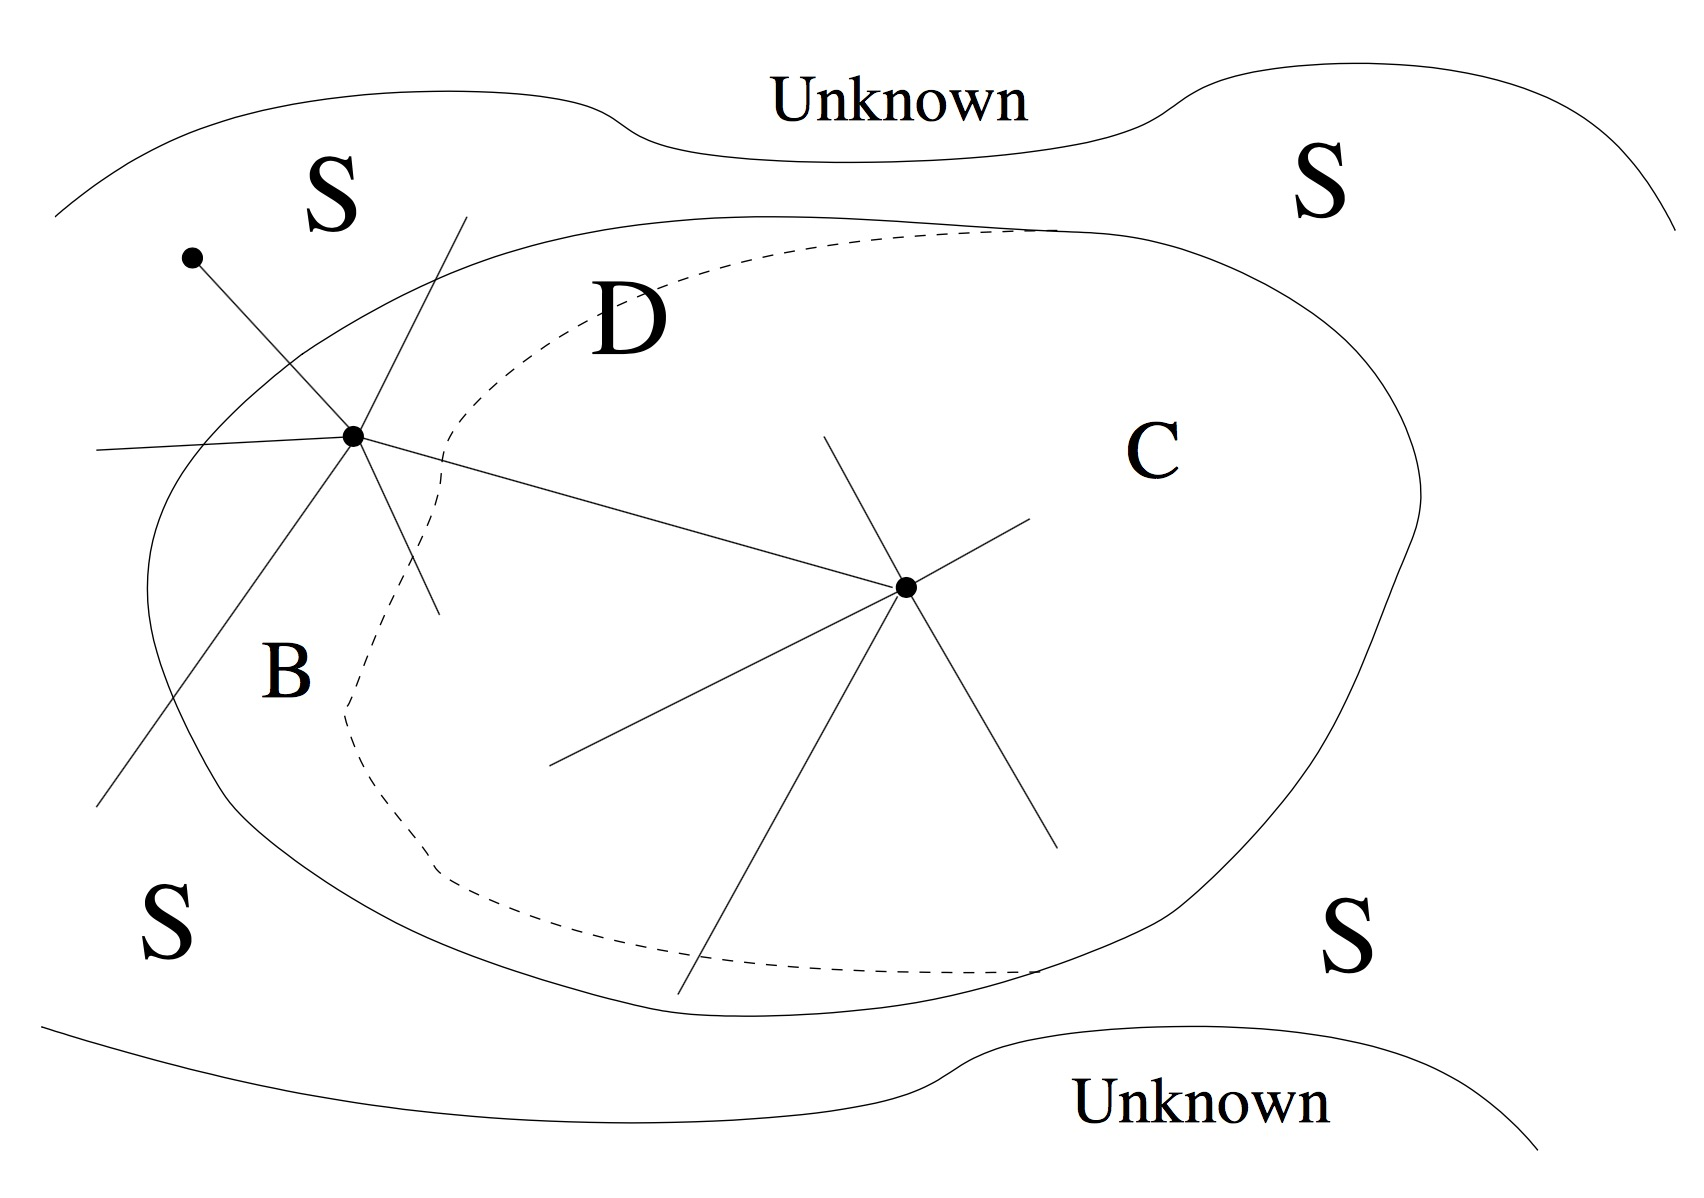
\includegraphics[scale = 0.09]{localCommunityDefinition.jpeg}
% %       \caption{Local Community Definition}
% %       \label{Local_Community_Definition}
%       \end{figure}

%     \column{0.5\textwidth}

% \begin{algorithm}[H]
%   \KwData{A social network $G$ and a start node $n_0$.}
%   \KwResult{A local community for $n_0$}% and its quality score R.
%   Add $n_0$ to $D$ and $B$, add all $\mathcal{V}_0$'s neighbors to $S$\;
%   %// \textbf{Discovery Phase}\;
%   \Repeat{$R^\prime \leq R$}{
% 	\For{each $n_i \in S$}{
%         Compute $R_i^\prime$\;
%     }
%     Find $n_i$ with the maximum $R_i^\prime$, breaking ties randomly\;
%     Add $n_i$ to $D$\;
%     Remove $n_i$ from $S$;
%     Update $B, S, R$\;
%   }
%    \Return{$\mathcal{D}$}
%   \caption{Original Local Community Identification Algorithm}
%    \end{algorithm}
%   \end{columns}

% \end{frame}


\begin{frame}{Local Community Detection - Previous Work}

\begin{columns}[T,onlytextwidth]
    \column{0.5\textwidth}
      \begin{figure}
      \centering
      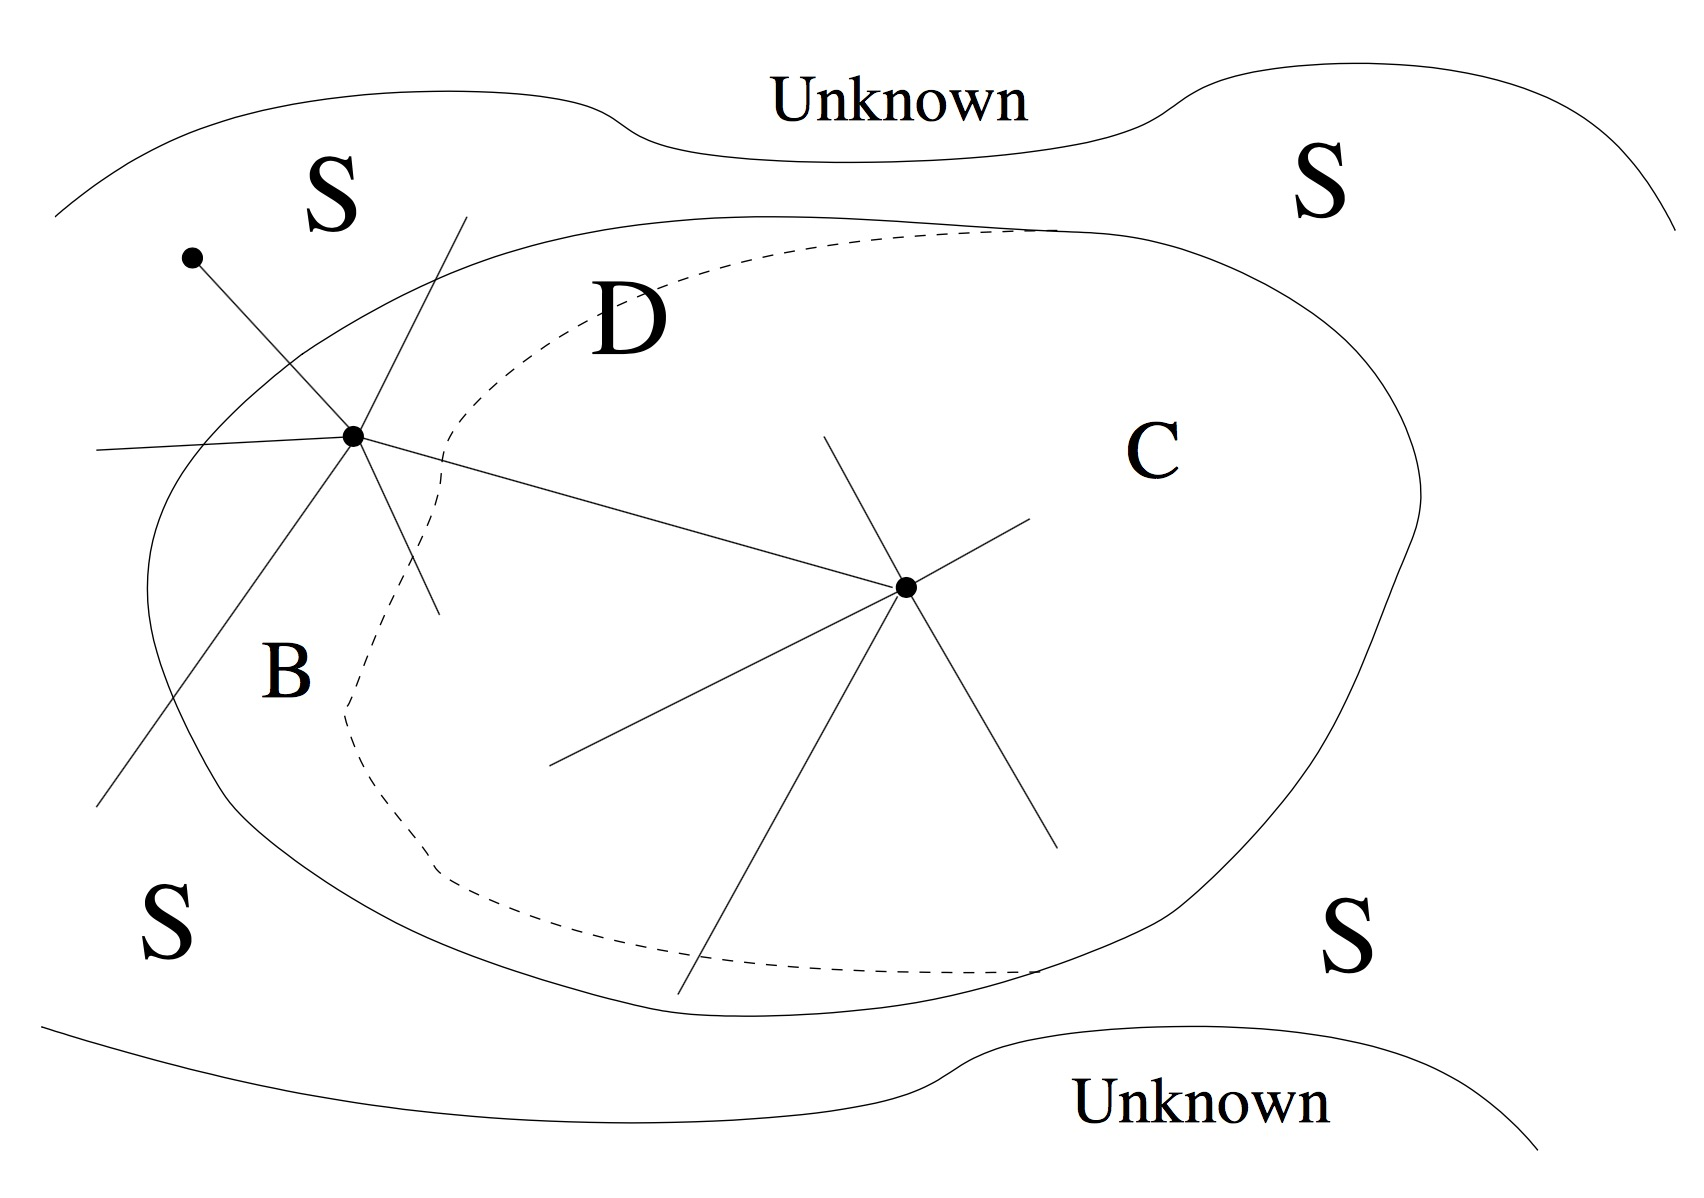
\includegraphics[scale = 0.08]{localCommunityDefinition.jpeg}
%       \caption{Local Community Definition}
%       \label{Local_Community_Definition}
      \end{figure}

    \column{0.5\textwidth}
     .
     
    \begin{equation}
    R = \frac{B_{\text{in\_edge}}}{B_{\text{out\_edge}}+B_{\text{in\_edge}}}
    \end{equation}
    
    ${B}_{in\_edge}$ is the number of edges that connect boundary nodes and other nodes in $\mathcal{D}$;  
    ${B}_{out\_edge}$ is the number of edges that connect boundary nodes and nodes in $\mathcal{S}$. 
    
  \end{columns}

\scriptsize
\begin{algorithm}[H]
  \KwData{A social network $G$ and a start node $n_0$.}
  \KwResult{A local community for $n_0$}% and its quality score R.
  Add $n_0$ to $D$ and $B$, add all $\mathcal{V}_0$'s neighbors to $S$\;
  %// \textbf{Discovery Phase}\;
  \Repeat{$R^\prime \leq R$}{
	\For{each $n_i \in S$}{
        Compute $R_i^\prime$\;
    }
    Find $n_i$ with the maximum $R_i^\prime$, breaking ties randomly\;
    Add $n_i$ to $D$\;
    Remove $n_i$ from $S$;
    Update $B, S, R$\;
  }
   \Return{$\mathcal{D}$}
  \caption{Original Local Community Identification Algorithm}
   \end{algorithm}


\end{frame}


\begin{frame}{Local Community Detection - Previous Work}
\small
\begin{equation}
\mathcal{UR} = \frac{\mathbb{E}(\mathcal{B}_{in\_edge})}{\mathbb{E}(\mathcal{B}_{in\_edge})+\mathbb{E}(\mathcal{B}_{out\_edge})}
\end{equation}
where $\mathbb{E}(\mathcal{B}_{in\_edge})$ is the expected number of edges that connect boundary nodes and other nodes in $\mathcal{D}$; while $\mathbb{E}(\mathcal{B}_{out\_edge})$ is the expected number of edges that connect boundary nodes and nodes in $\mathcal{S}$.


\begin{columns}[T,onlytextwidth]
    \column{0.6\textwidth}
      \begin{figure}
      \centering
      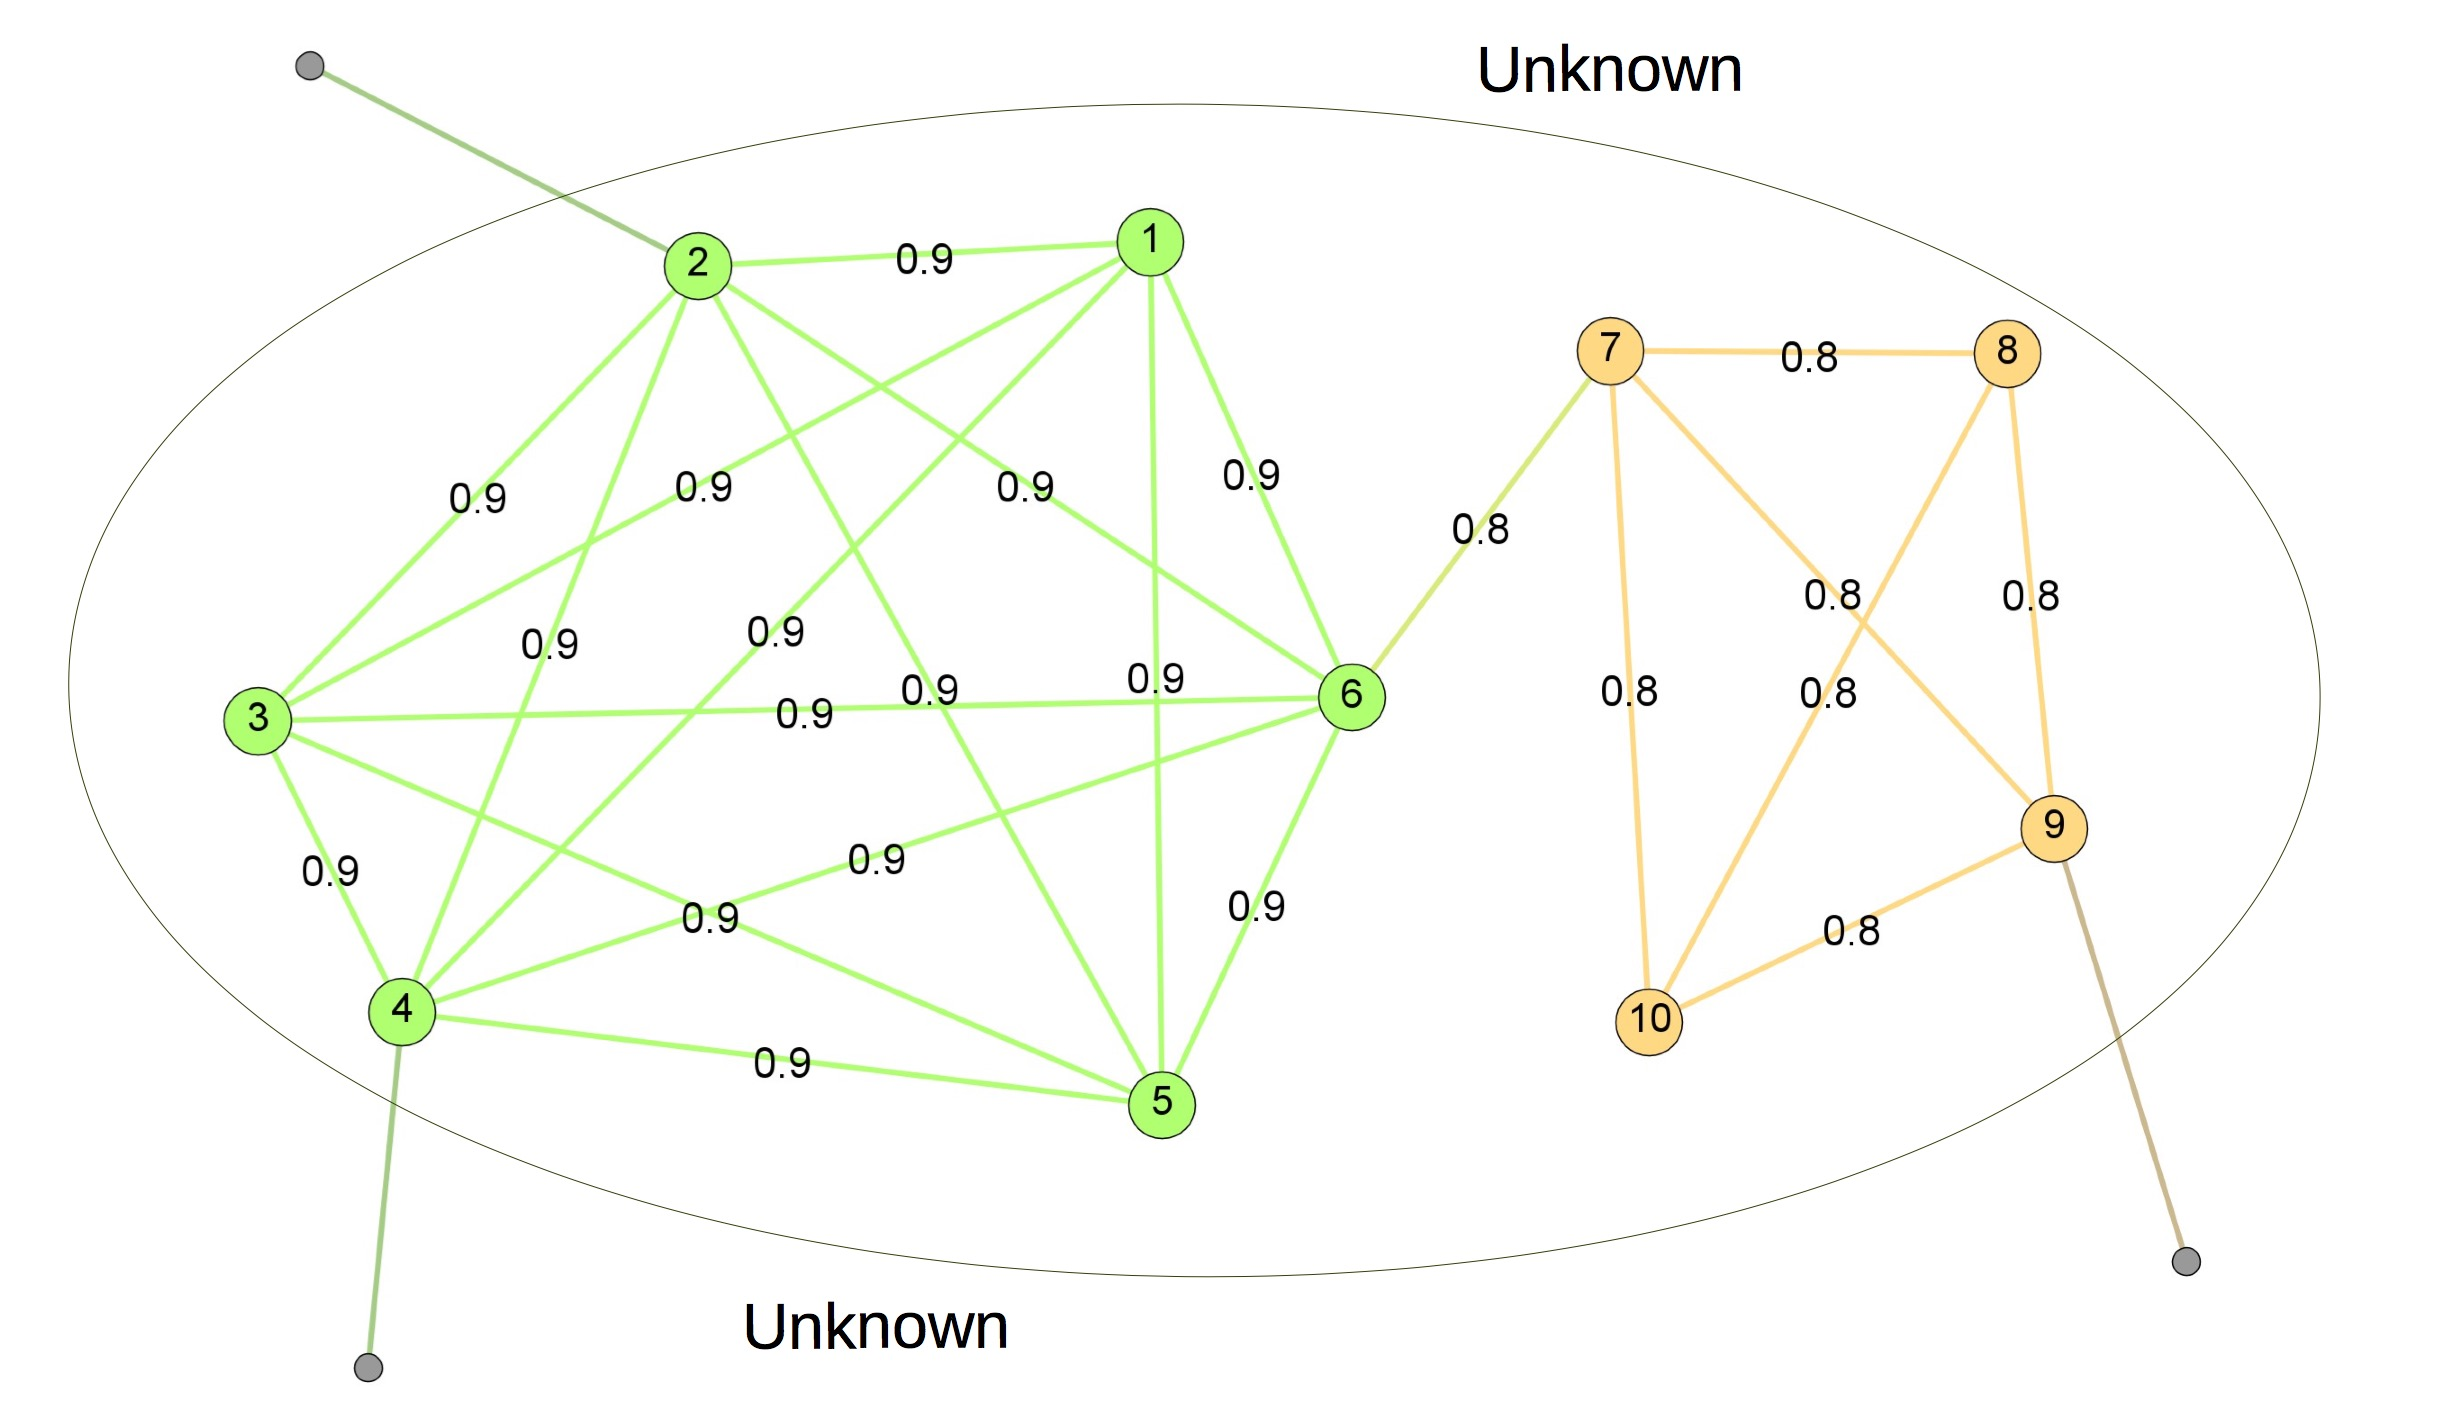
\includegraphics[scale = 0.075]{toy_example.jpeg}
      \caption{An example showing the problem of only using $\mathcal{UR}$ to find the local community.}
      \label{problem_example}
      \end{figure}

    \column{0.4\textwidth}
    .
    
     The $\mathcal{UR}$ of the community, after adding $\mathcal{V}_1, \mathcal{V}_3$ or $\mathcal{V}_5$, are all 
\begin{align*}
\frac{0.9}{4\times0.9+(4\times0.9+0.8)+0.9}=0.1011
\end{align*}
\newline
After adding node $\mathcal{V}_2$ or $\mathcal{V}_4$, the $\mathcal{UR}$ will be less than 0.1011 due to extra outward edges. The $\mathcal{UR}$ of the community after adding node $\mathcal{V}_7$ is 
\begin{align*}
\frac{0.8}{5\times0.9+3\times0.8+0.8}=0.1039
\end{align*}
    
  \end{columns}

\end{frame}

\begin{frame}{Local Community Detection - Previous Work}

\end{frame}


\begin{frame}{Local Community Detection - Algorithm}
  \scriptsize
\begin{algorithm}[H]
  \KwData{A network $\mathcal{G}$, a start node $\mathcal{V}_0$ and number of steps $\lambda$.}
  \KwResult{A local community for $\mathcal{V}_0$}% and its quality score R.
  Add $\mathcal{V}_0$ to $\mathcal{D}$ and $\mathcal{B}$, add all $\mathcal{V}_0$'s neighbors to $S$, $\mathcal{UR} \leftarrow 0$\;
  %// \textbf{Discovery Phase}\;
  \Repeat{no new node is added to $\mathcal{D}$}{
  	Array $nodelist \leftarrow [ ]$\;
	\For{each $\mathcal{V}_i \in S$}{
        Compute $\mathcal{UR}_i$; // $\mathcal{UR}_i$ represents the $\mathcal{UR}$ value after adding node $\mathcal{V}_i$\;
        Compute $\mathcal{K}_i$\;
        Add $\mathcal{V}_i$ to $nodelist$\;
%         \If{$\mathcal{V}_i.K>threshold$}{
%         	Add $\mathcal{V}_i$ to $nodelist$\;
%         }
    }
        %Sort the node $\mathcal{V}_i \in S$ first by $K_i$, second by $R_i$\;
        \uIf{$|\mathcal{D}|<\lambda$}{
        Sort $nodelist$ first by $\mathcal{K}_i$, then by $\mathcal{UR}_i$\;}
        \Else{
        Sort $nodelist$ first by $\mathcal{UR}_i$, then by $\mathcal{K}_i$\;}
%         // If some nodes have same $\mathcal{K}_i$ and $\mathcal{UR}_i$, break ties randomly\;
    \For{each $\mathcal{V}_i \in nodelist$}{
    	\If{$\mathcal{UR}_i>\mathcal{UR}$}{
        	$\mathcal{UR} \leftarrow \mathcal{UR}_i$\;
        	Add $\mathcal{V}_i$ to $\mathcal{D}$; Remove $\mathcal{V}_i$ from $\mathcal{S}$\;
            Update $\mathcal{B}$, $\mathcal{D}$\;
            Update shell nodes possibility based on Equation (10)\;
            \textbf{break} for loop
        }
    }
  }
   \Return{$\mathcal{D}$}
  \caption{Local Community Identification with Edge Uncertainty}
   \end{algorithm}

\end{frame}


\section{Introduction}
\subsection{Background}
\begin{frame}[fragile]{Background}

%  The \themename theme is a Beamer theme with minimal visual noise
%  inspired by the \href{https://github.com/hsrmbeamertheme/hsrmbeamertheme}{\textsc{hsrm} Beamer
%  Theme} by Benjamin Weiss.

%  Enable the theme by loading

 % \begin{verbatim}    \documentclass{beamer}
 %   \usetheme{metropolis}\end{verbatim}

%  Note, that you have to have Mozilla's \emph{Fira Sans} font and XeTeX
 % installed to enjoy this wonderful typography.

In graph theory, \textbf{centrality} identifies the importance of vertices within a graph.
%, which is depicted by \textbf{shortest path}
\vspace{-0.11in}
\begin{figure}[H]
\centering
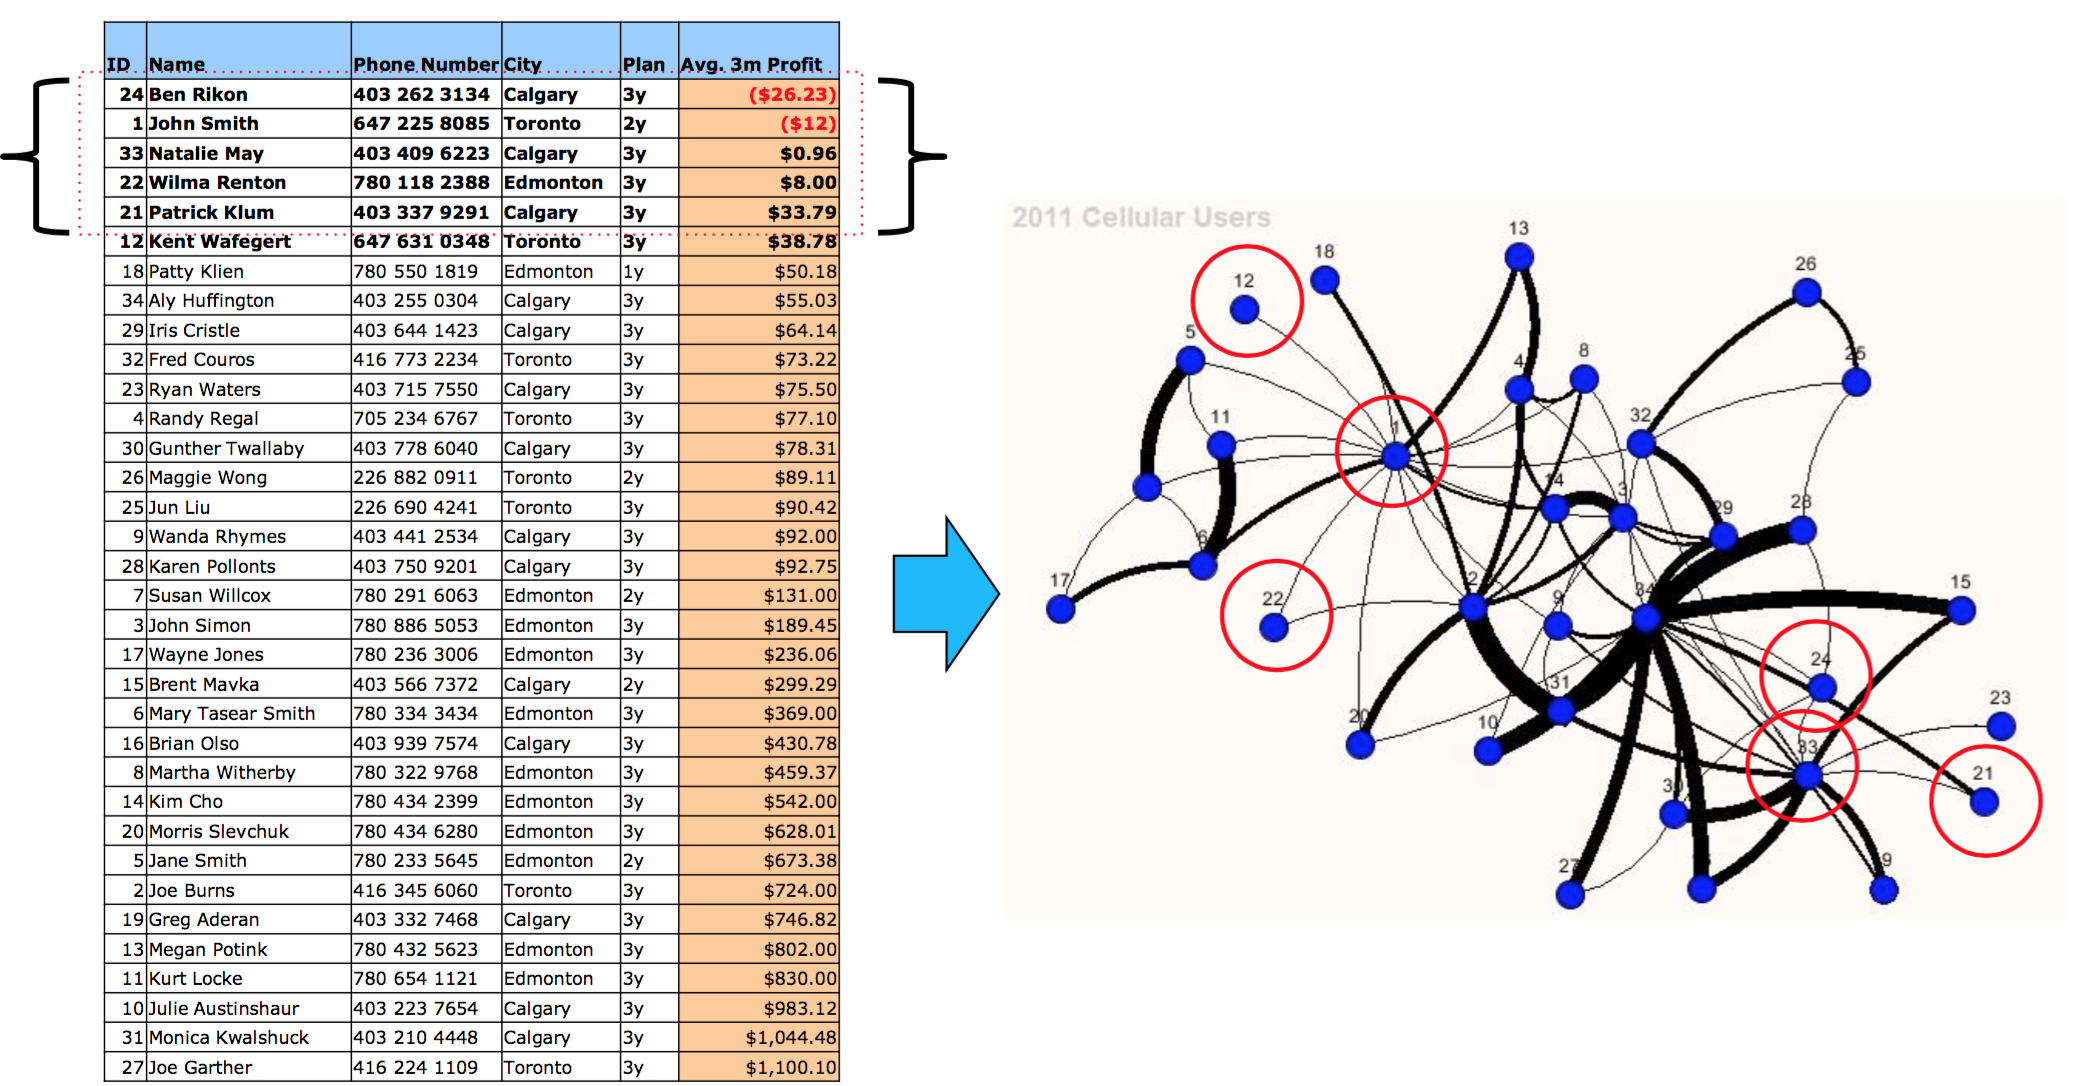
\includegraphics[scale = 0.29]{famous_example.png}
\caption{An example illustrating identifying the most influential person in a social network via centrality}
%\label{famous_example}
\end{figure}
\end{frame}

\begin{frame}
\frametitle{Background: Centrality}

\textbf{Betweenness Centrality}: Measures how many times a node n occurs in a shortest path between any other 2 nodes in the graph;

\textbf{Closeness Centrality}: Mean shortest path distance between a node n and all other nodes reacheable from it;

\end{frame}

%\begin{frame}

%\begin{frame}
%\frametitle{Background: Betweenness Centrality [Wikipedia]}

%The \textbf{betweenness centrality} of a vertex $v$ in a graph $G:=(V,E)$ with $V$ vertices is computed as follows:
%\begin{itemize}
%\item For each pair of vertices $(i,j)$, compute all the \textbf{shortest paths} between them
%\item For each pair of vertices $(i,j)$, determine the \textbf{fraction of shortest paths} that pass through the vertex in question (here, vertex $v$)
%\item Sum this fraction over all pairs of vertices $(i,j)$
%\begin{equation*}
%C_B(v) = \sum_{i\neq v \neq j \in V}\frac{\sigma_{ij}(v)}{\sigma_{ij}}
%\end{equation*}
%\begin{itemize}
%\item $\sigma_{ij}$ is the total number of shortest paths from node $i$ to node $j$ and $\sigma_{ij}(v)$ is the number of those paths that pass through $v$
%\end{itemize}

%\end{itemize}


%\end{frame}

%\begin{frame}
%\frametitle{Background: Closeness Centrality [Wikipedia]}
%   Sections group slides of the same topic

%   \begin{verbatim}    \section{Elements}\end{verbatim}

%   for which \themename provides a nice progress indicator \ldots

%In a connected graph, the \textbf{closeness centrality} of a node is the average length of the \textbf{shortest path} between the node and all other nodes in the graph. Thus the more central a node is, the closer it is to all other nodes.
%\begin{equation*}
%C_C(i) = \frac{1}{\sum_{j}d_{ij}}
%\end{equation*}
%\begin{itemize}
%\item $d_{ij}$ is the \textbf{shortest distance} between vertices $i$ and $j$
%\end{itemize}

%\end{frame}

\subsection{Motivation}
\begin{frame}
\frametitle{Motivation: Uncertainty}
\begin{itemize}
\item Traditional graph centrality measures are applied to discrete, static graphs, where binary edges represent the "presence" or "absence" of a relationship
\item In practice, however, edge uncertainty arises almost everywhere:
\begin{itemize}
\item When considering the evolution of networks overtime, there is inherent uncertainty about the strength of underlying relationships at a particular point in time
\item Even in static graphs, it is sometimes uncertain whether the interaction between two nodes is existed, eg. protein-protein interaction network, crime evidence network, etc.
\end{itemize}
\end{itemize}
\end{frame}

\begin{frame}
\frametitle{Motivation: Probabilistic Graph}
\begin{figure}[H]
\centering
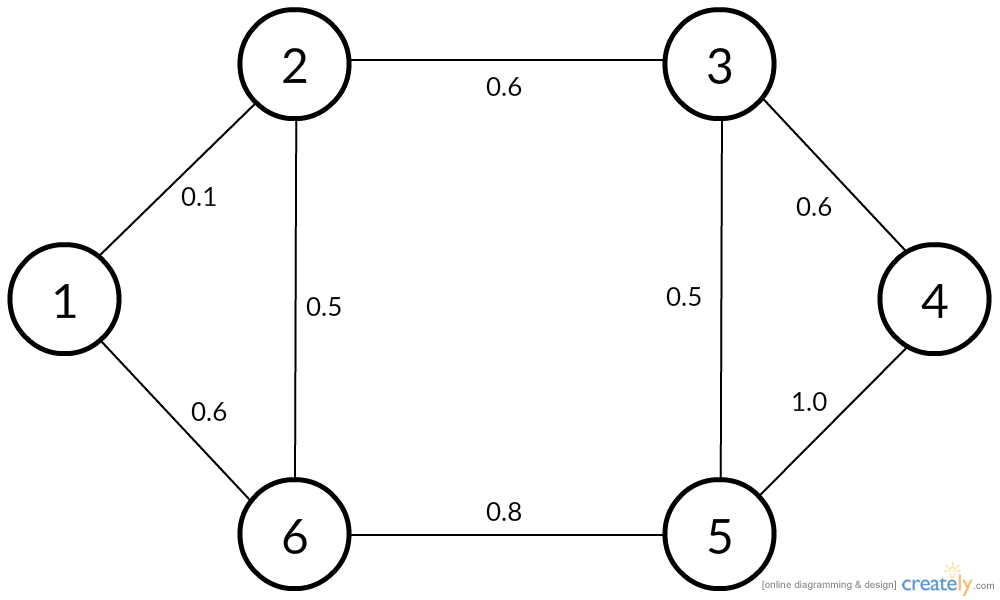
\includegraphics[scale = 0.2]{probabilistic_graph.png}
\caption{An example of probabilistic graph}
%\label{probabilistic_graph}
\end{figure}
\vspace{-0.28in}
This leads to the question that we are looking at: \textbf{Given a probabilistic graph $G := (V,E,P,W)$, where $V$ is a set of vertices, $P$ is the probability distribution over edges $E$, $W$ is the edge attributes, usually weight, how do we compute centrality measures with the presence of edge uncertainty?}
\end{frame}

\section{Related Work}
\subsection{Negative Logarithm \cite{potamias2009nearest}}
\begin{frame}{Negative Logarithm \cite{potamias2009nearest}}
% 	\themename supports 4 different titleformats:
% 	\begin{itemize}
% 		\item Regular
% 		\item \textsc{Smallcaps}
% 		\item \textsc{allsmallcaps}
% 		\item ALLCAPS
% 	\end{itemize}
% 	They can either be set at once for every title type or individually.
\begin{itemize}
\item A simple approach is to consider the probabilities
as costs by taking the negative logarithm of the probability; the weight between two adjacent vertices $i$ and $j$ are defined as follow:
\begin{equation*}
W(e_{uv}) = -log(P(e_{uv}))
\end{equation*}
\vspace{-0.2in}
\begin{itemize}
\item $P(e_{uv})$ is the probability defined on edge $e_{uv}$
\item $W(e_{uv})$ is the new weight defined by the negative logarithm of edge probability
\end{itemize}
\item Thus probabilities are converted to weights and all existential graph mining methods on discrete graphs become accessible under this framework
\end{itemize}
\end{frame}

% {
%     \metroset{titleformat frame=smallcaps}
% \begin{frame}{Small caps}
% 	This frame uses the \texttt{smallcaps} titleformat.

% 	\begin{alertblock}{Potential Problems}
% 		Be aware, that not every font supports small caps. If for example you typeset your presentation with pdfTeX and the Computer Modern Sans Serif font, every text in smallcaps will be typeset with the Computer Modern Serif font instead.
% 	\end{alertblock}
% \end{frame}
% }
\subsection{Most Probable Path \cite{pfeiffer2010probabilistic}, \cite{pfeiffer2011methods}}
\begin{frame}{Most Probable Path \cite{pfeiffer2010probabilistic}, \cite{pfeiffer2011methods}}
\begin{itemize}
\item Using the notion of probabilistic paths, we calculate the probability of the existence of a path $\rho_{ij}$ between nodes $i$ and $j$ as follows:
\begin{equation*}
P(\rho_{ij}) = \prod_{e_{uv} \in E}P(e_{uv})
\end{equation*}
\vspace{-0.12in}
\begin{itemize}
\item $e_{uv}$ is the edge connecting two adjacent nodes $u$ and $v$
\end{itemize}
\item Now given two nodes $i$ and $j$, the \textbf{most probable path} is simply the one with \textit{maximum likelihood}:
\[ \rho_{ij}^{ML} = argmaxP(\rho_{ij}) \]
\item Then we can compute the most probable path by applying Dijkstra's shortest path algorithm, but expanding on the most probable path instead
\end{itemize}
\end{frame}

% {
% \metroset{titleformat frame=allsmallcaps}
% \begin{frame}{All small caps}
% 	This frame uses the \texttt{allsmallcaps} titleformat.

% 	\begin{alertblock}{Potential problems}
% 		As this titleformat also uses smallcaps you face the same problems as with the \texttt{smallcaps} titleformat. Additionally this format can cause some other problems. Please refer to the documentation if you consider using it.

% 		As a rule of thumb: Just use it for plaintext-only titles.
% 	\end{alertblock}
% \end{frame}
% }

% {
% \metroset{titleformat frame=allcaps}
% \begin{frame}{All caps}
% 	This frame uses the \texttt{allcaps} titleformat.

% 	\begin{alertblock}{Potential Problems}
% 		This titleformat is not as problematic as the \texttt{allsmallcaps} format, but basically suffers from the same deficiencies. So please have a look at the documentation if you want to use it.
% 	\end{alertblock}
% \end{frame}
% }

\section{Our Approach}
\begin{frame}[fragile]{Inversed Probabilistic Graph}
%       \begin{verbatim}The theme provides sensible defaults to
% \emph{emphasize} text, \alert{accent} parts
% or show \textbf{bold} results.\end{verbatim}

%   \begin{center}becomes\end{center}

%   The theme provides sensible defaults to \emph{emphasize} text,
%   \alert{accent} parts or show \textbf{bold} results.

To circumvent the relatively heavy computation of \textit{Most Probable Path} method and the low accuracy of \textit{Negative Logarithm} method, we propose a new approach, \textbf{Inversed Probabilistic Graph}, defined as follows:
\begin{itemize}
\item Given a probabilistic graph $G:=(V,E,P,W)$, for an edge $e_{uv}$, we can convert probability to weight by taking the inverse of edge probability
\[ W'(e_{uv}) = \frac{W(e_{uv})}{P(e_{uv})^\lambda }\]
\vspace{-0.15in}
\begin{itemize}
\item Here $\lambda$ is a hyper-parameter, $W'$ is the newly computed weight for an edge
\item In experiment we use $\lambda = 0.4$
\end{itemize}
\end{itemize}
Again, we can apply existential graph mining algorithms under this framework
\end{frame}

\section{Experiment Results}


\begin{frame}
\frametitle{Illustrative Experiment}
\begin{itemize}
\item Firstly, we draw two graphs, each demonstrating the centrality ranking evolution of selected individuals in the Enron dataset, as \textit{Pfeiffer et al} did in \cite{pfeiffer2010probabilistic}, \cite{pfeiffer2011methods}

\item We evaluate our method by looking at each graph if centrality evolutions correspond to the background provided in the Enron dataset


\end{itemize}
\end{frame}

\begin{frame}
\frametitle{Centrality Ranking over Time in Enron: Lay and Skilling}
\begin{figure}[H]
\centering
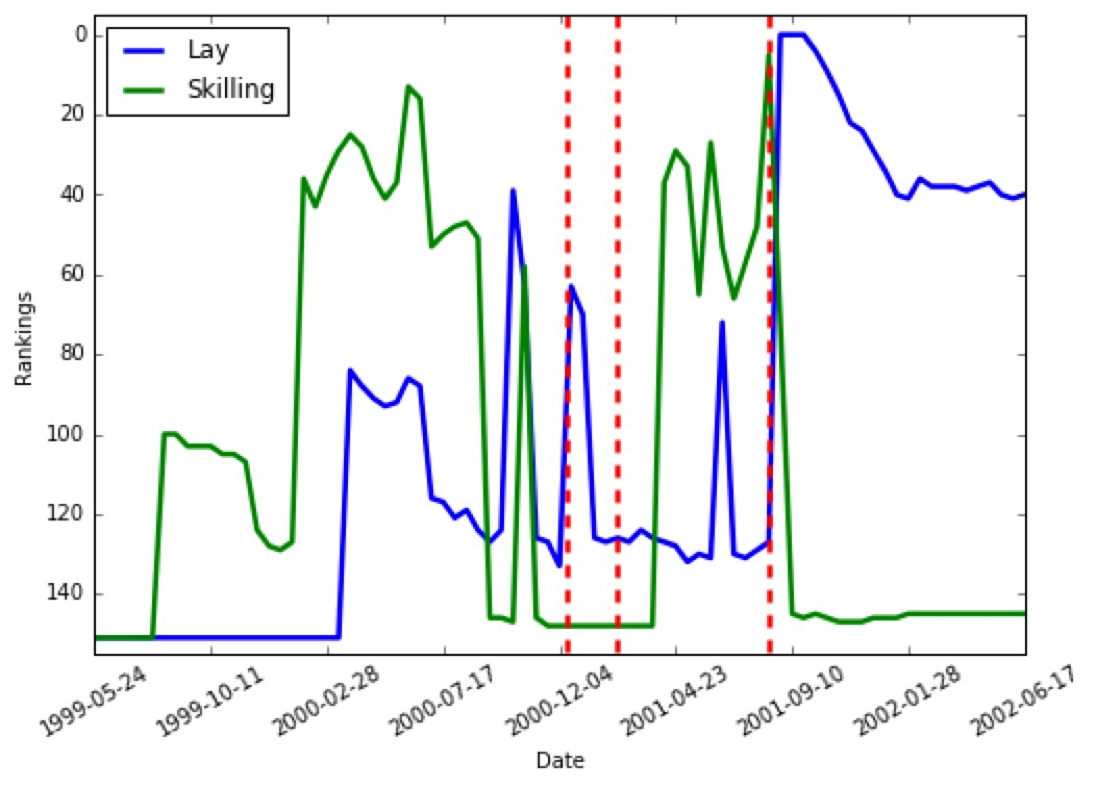
\includegraphics[scale = 0.3]{rank_change1.png}
\caption{Centrality ranking evolution of Lay and Skilling}
%\label{probabilistic_graph}
\end{figure}
\vspace{-0.15in}
\begin{itemize}
\item On December $13^{th}$, 2000, it was announced that Skilling would assume the CEO position at Enron, with Lay retiring but remaining as a chairman.
\item During February 2001, Skilling made the transition to CEO and Lay retired
\item On August $14^{th}$, 2001, Skilling resigned from the position of CEO and Lay took over
\end{itemize}
\end{frame}


\begin{frame}
\frametitle{Centrality Ranking over Time in Enron: Kitchen and Lavorato}
\begin{figure}[H]
\centering
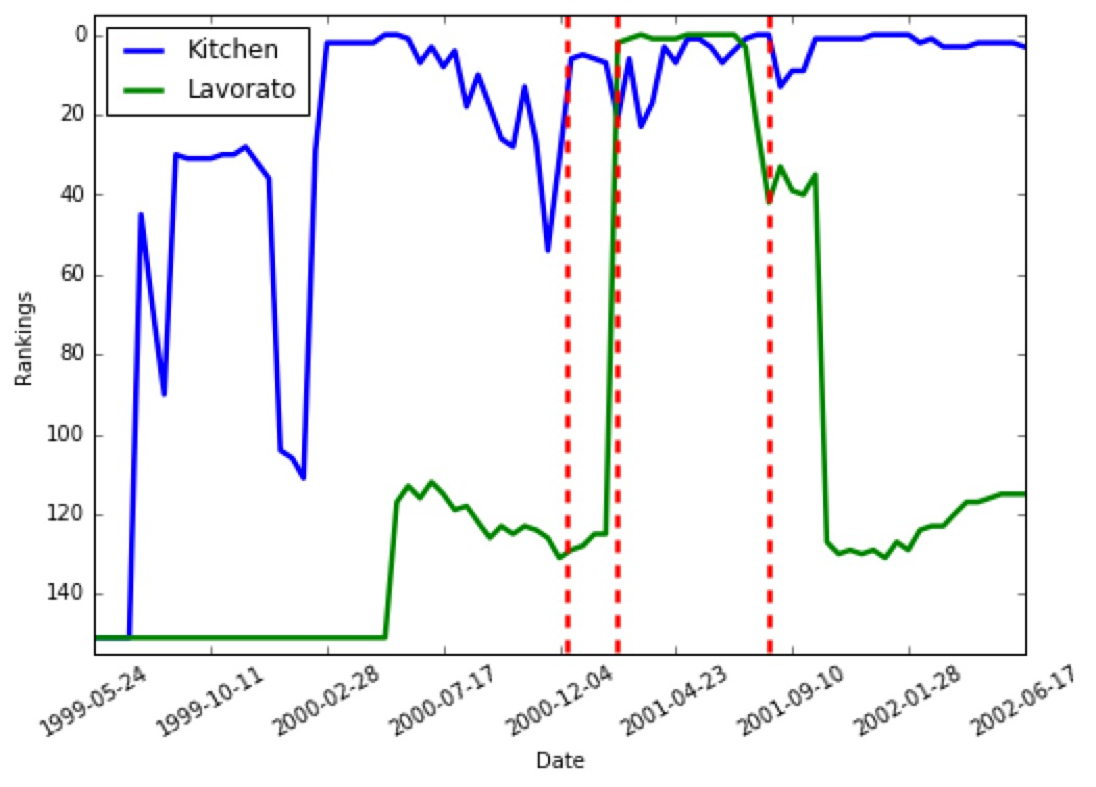
\includegraphics[scale = 0.3]{rank_change2.png}
\caption{Centrality ranking evolution of Kitchen and Lavorato}
%\label{probabilistic_graph}
\end{figure}
\vspace{-0.15in}
\begin{itemize}
\item Kitchen and Lavorato were executives for Enron Americas
\item Lavorato is only important during Skilling's tenure as CEO; his centrality drops noticeably otherwise. This suggests that Skilling and Lavorato were extremely close
\item On the other hand, Kitchen had extremely high rankings throughout
\end{itemize}
\end{frame}

\begin{frame}
\frametitle{Comparative Experiment}
\begin{itemize}
\item Secondly, we compare the two methods, \textit{Negative Logarithm} and \textit{Most Probable Path} that are illustrated above, with our method on 
\begin{itemize}
\item Enron dataset
\item Simulated weighted graph dataset and discrete unweighted graph dataset
\end{itemize}
\item We evaluate each method via visualizing the linear relationship between centrality rankings computed by each method and average centrality rankings computed by sampling
\item The stronger linear relationship that a plot indicates, the better performance the method is.
\item The metric of the linear relationship strength:
\[ r=\frac{\sum_{i=1}^{m}|x_i-y_i|}{\sqrt{2}m} \]
\end{itemize}
\end{frame}



\begin{frame}
\frametitle{Centralities on Enron Dataset}
\vspace{0.15in}
\begin{figure}[H]
\centering
\begin{subfigure}{.32\textwidth}
  \centering
  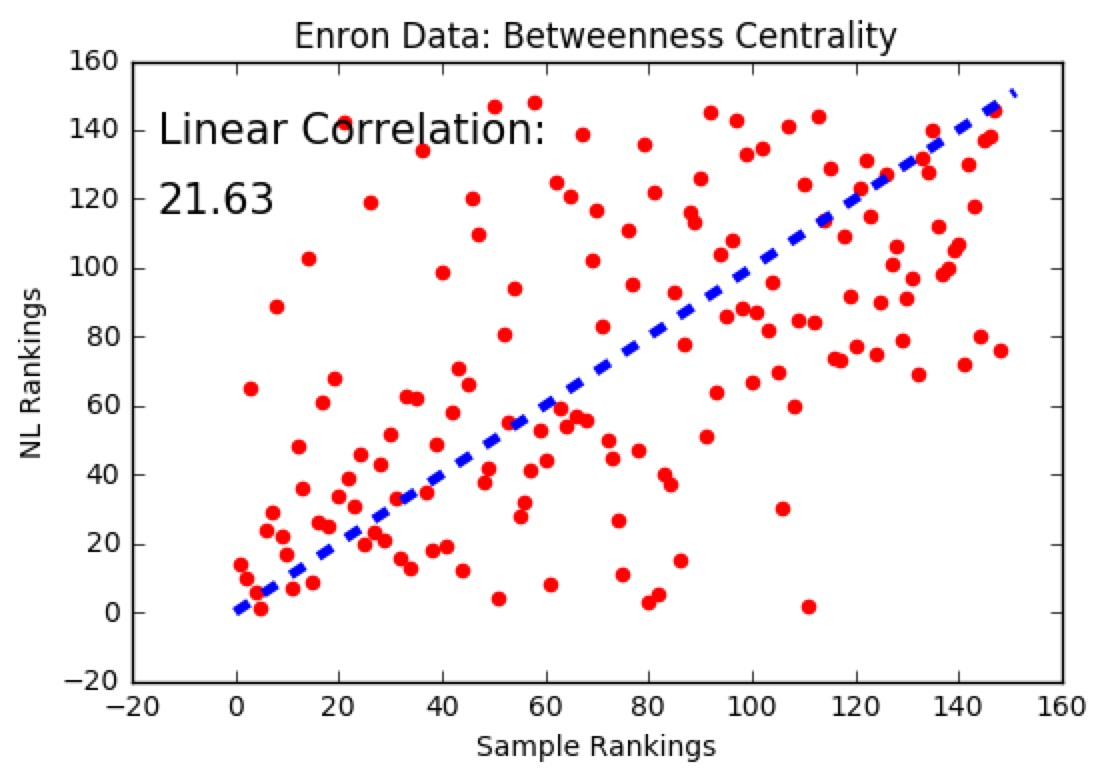
\includegraphics[width=0.95\linewidth]{EBC_NL.jpeg}
%  \caption{Per-map suboptimality}
%  \label{acpermap}
\end{subfigure}
%\caption{Normalized mean suboptimality on the per-map and uni-map bases for GBDT, SVM, and NN classifiers using AlexNet as a feature extractor}
\begin{subfigure}{.32\textwidth}
	\centering
    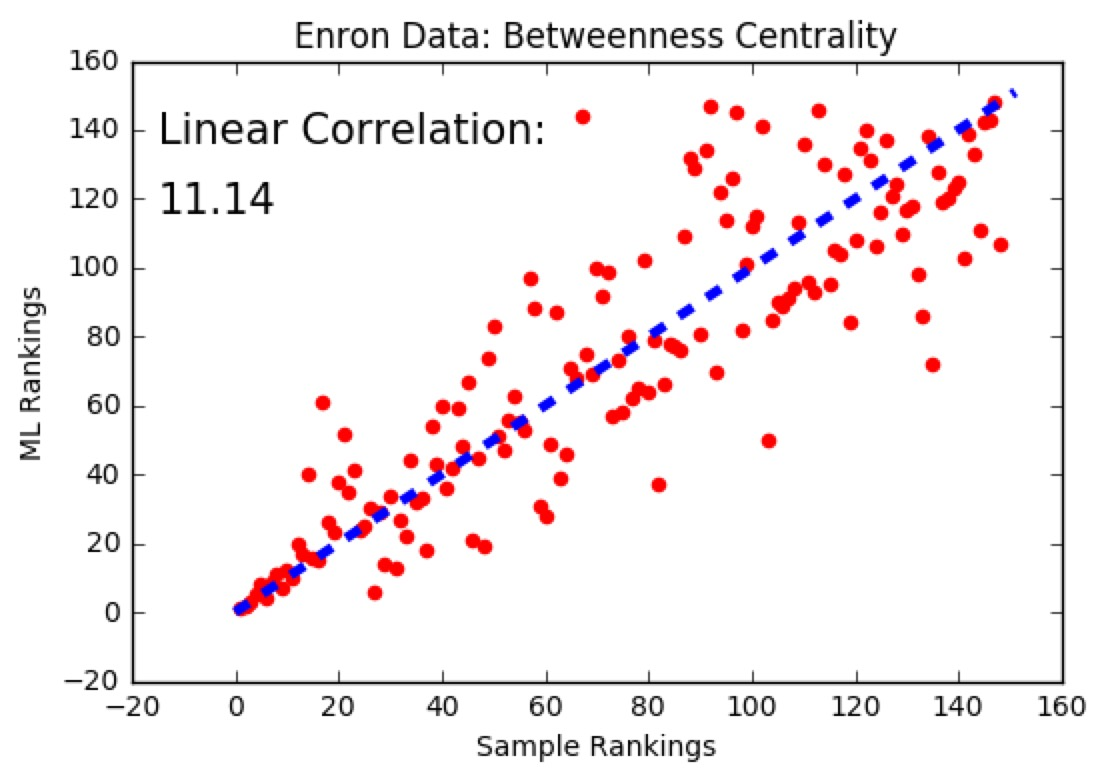
\includegraphics[width=0.95\linewidth]{EBC_ML.jpeg}
\end{subfigure}
%\label{alexclass}
\begin{subfigure}{.32\textwidth}
	\centering
    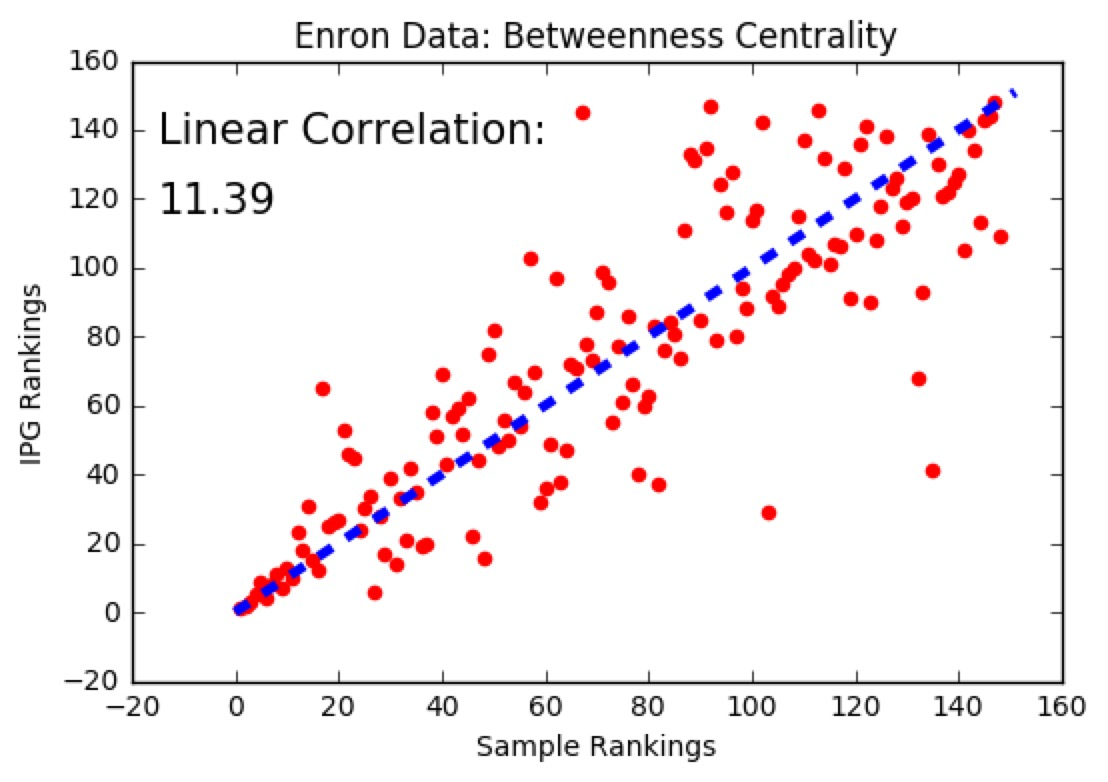
\includegraphics[width=0.95\linewidth]{EBC_IPG.jpeg}
\end{subfigure}
\caption{Comparison of betweenness centralities computed by different methods on Enron dataset}
\end{figure}
\vspace{-0.1in}
\begin{figure}[H]
\centering
\begin{subfigure}{.32\textwidth}
  \centering
  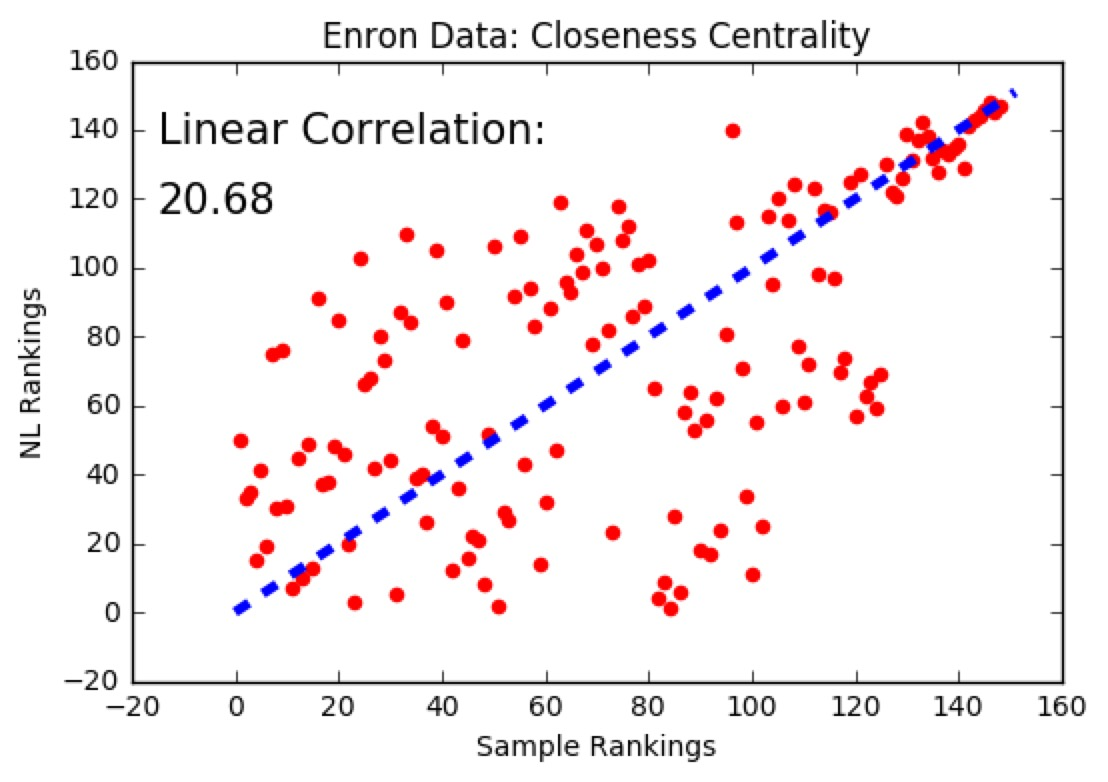
\includegraphics[width=0.95\linewidth]{ECC_NL.jpeg}
%  \caption{Per-map suboptimality}
%  \label{acpermap}
\end{subfigure}
%\caption{Normalized mean suboptimality on the per-map and uni-map bases for GBDT, SVM, and NN classifiers using AlexNet as a feature extractor}
\begin{subfigure}{.32\textwidth}
	\centering
    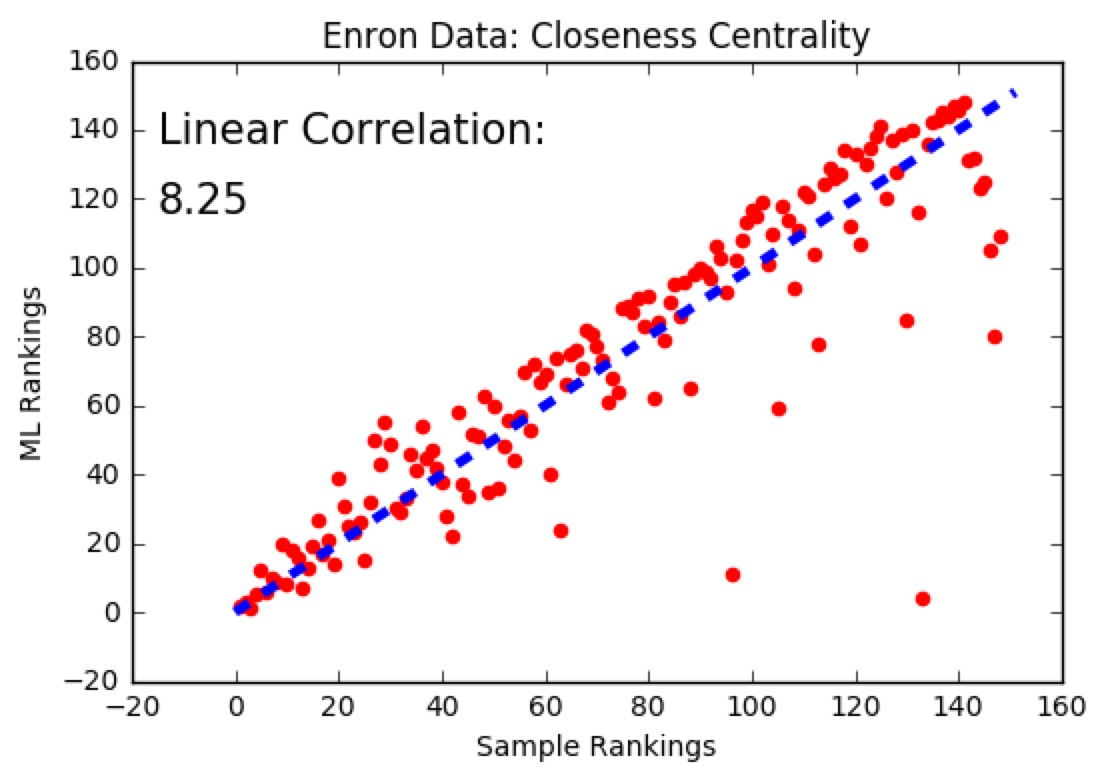
\includegraphics[width=0.95\linewidth]{ECC_ML.jpeg}
\end{subfigure}
%\label{alexclass}
\begin{subfigure}{.32\textwidth}
	\centering
    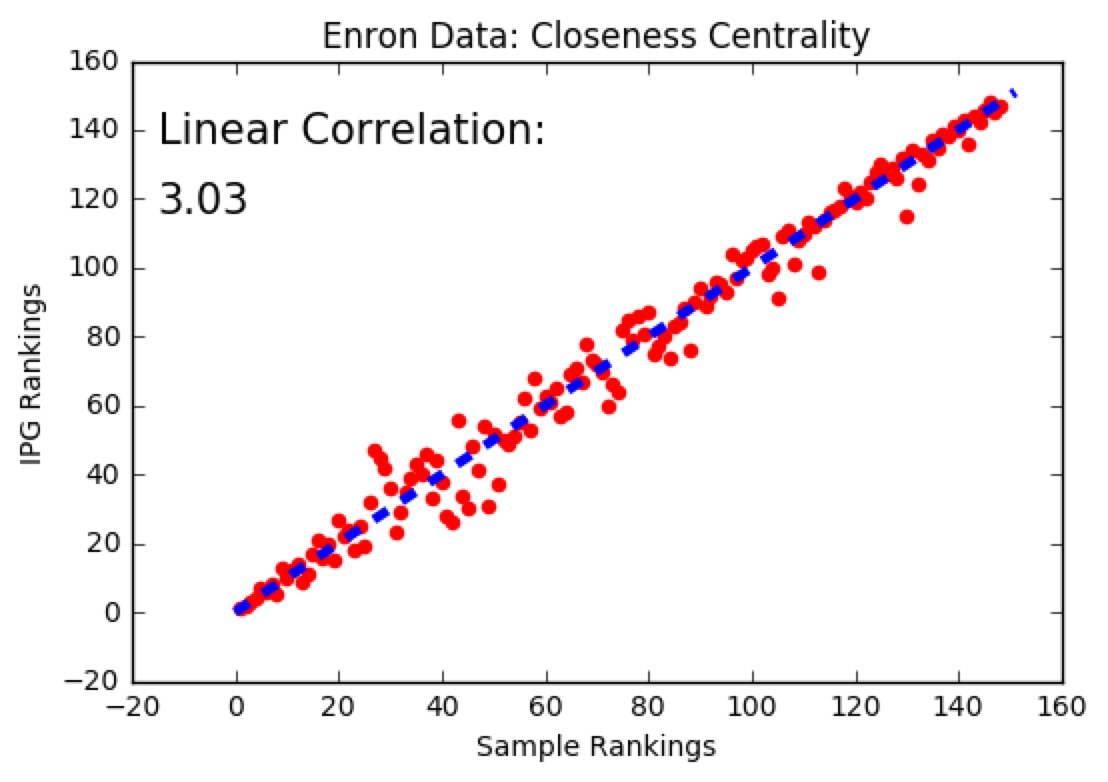
\includegraphics[width=0.95\linewidth]{ECC_IPG.jpeg}
\end{subfigure}
\caption{Comparison of closeness centralities computed by different methods on Enron dataset}
\end{figure}
%\caption{Betweenness Centrality on Enron Dataset}
\end{frame}



\begin{frame}
\frametitle{Centralities on Simulated Unweighted Graphs}
\vspace{0.15in}
\begin{figure}[H]
\centering
\begin{subfigure}{.32\textwidth}
  \centering
  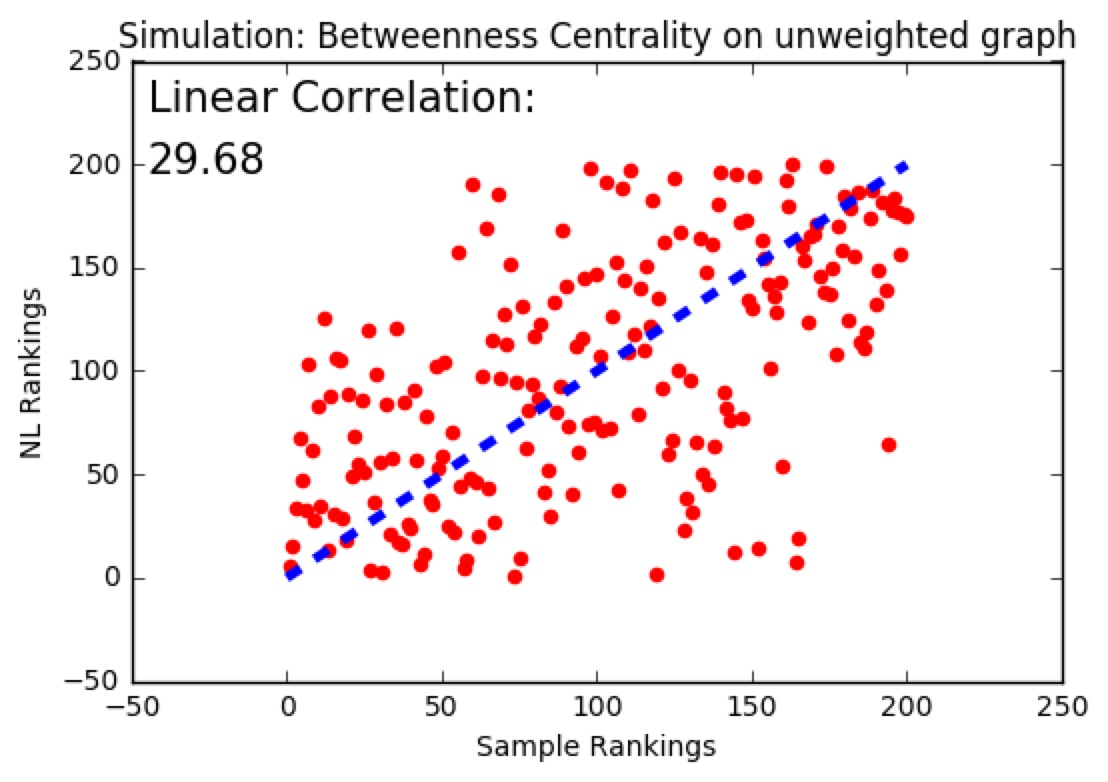
\includegraphics[width=0.95\linewidth]{BCU_NL.jpeg}
%  \caption{Per-map suboptimality}
%  \label{acpermap}
\end{subfigure}
%\caption{Normalized mean suboptimality on the per-map and uni-map bases for GBDT, SVM, and NN classifiers using AlexNet as a feature extractor}
\begin{subfigure}{.32\textwidth}
	\centering
    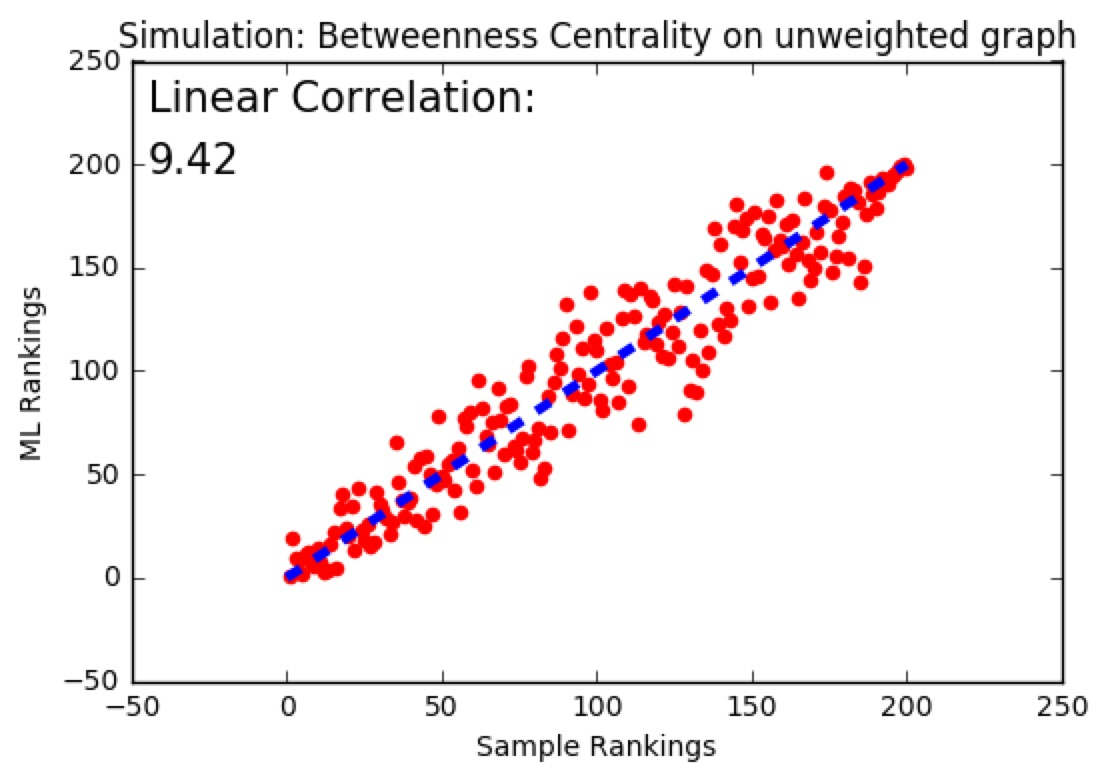
\includegraphics[width=0.95\linewidth]{BCU_ML.jpeg}
\end{subfigure}
%\label{alexclass}
\begin{subfigure}{.32\textwidth}
	\centering
    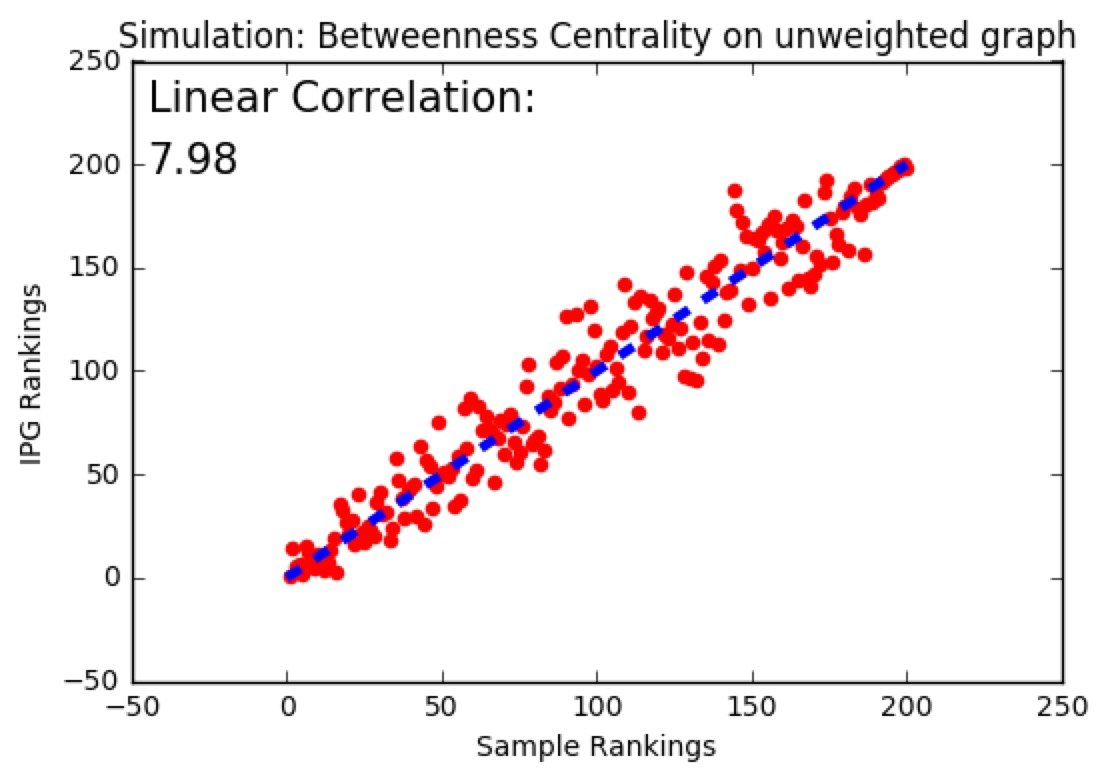
\includegraphics[width=0.95\linewidth]{BCU_IPG.jpeg}
\end{subfigure}
\caption{Comparison of betweenness centralities computed by different methods on simulated unweighted graphs}
\end{figure}
\vspace{-0.1in}
\begin{figure}[H]
\centering
\begin{subfigure}{.32\textwidth}
  \centering
  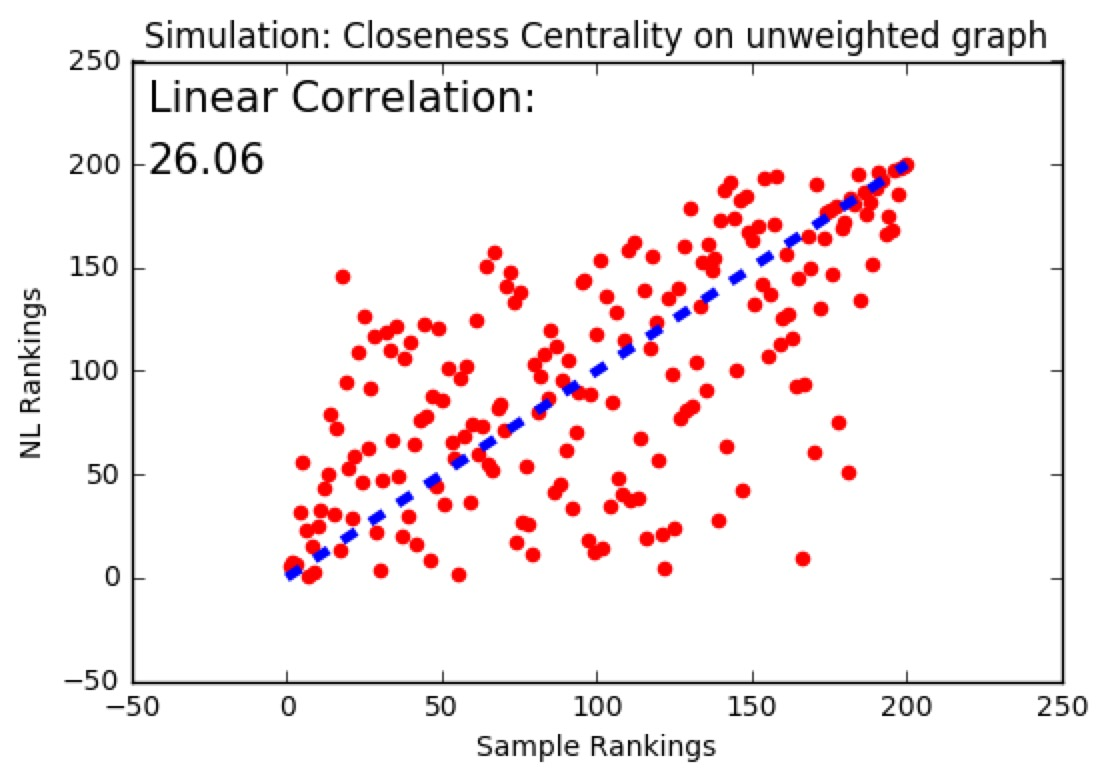
\includegraphics[width=0.95\linewidth]{CCU_NL.jpeg}
%  \caption{Per-map suboptimality}
%  \label{acpermap}
\end{subfigure}
%\caption{Normalized mean suboptimality on the per-map and uni-map bases for GBDT, SVM, and NN classifiers using AlexNet as a feature extractor}
\begin{subfigure}{.32\textwidth}
	\centering
    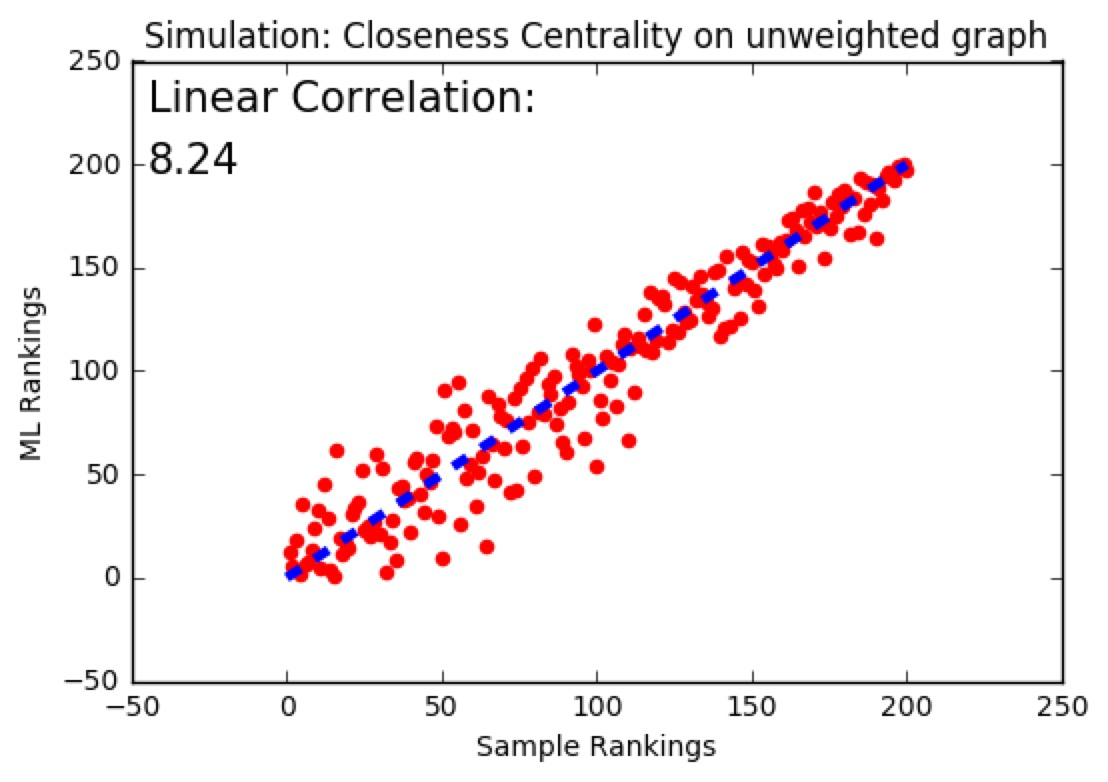
\includegraphics[width=0.95\linewidth]{CCU_ML.jpeg}
\end{subfigure}
%\label{alexclass}
\begin{subfigure}{.32\textwidth}
	\centering
    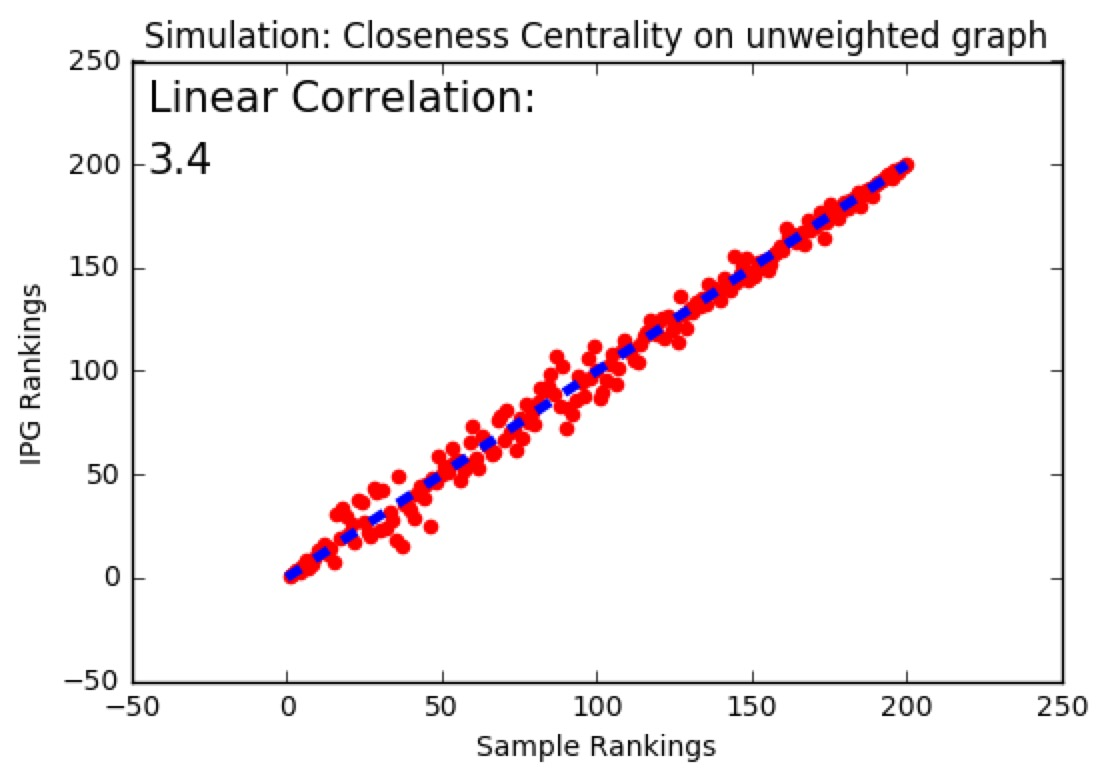
\includegraphics[width=0.95\linewidth]{CCU_IPG.jpeg}
\end{subfigure}
\caption{Comparison of closeness centralities computed by different methods on simulated unweighted graphs}
\end{figure}
%\caption{Betweenness Centrality on Enron Dataset}
\end{frame}


\begin{frame}
\frametitle{Centralities on Simulated Weighted Graphs}
\vspace{0.15in}
\begin{figure}[H]
\centering
\begin{subfigure}{.32\textwidth}
  \centering
  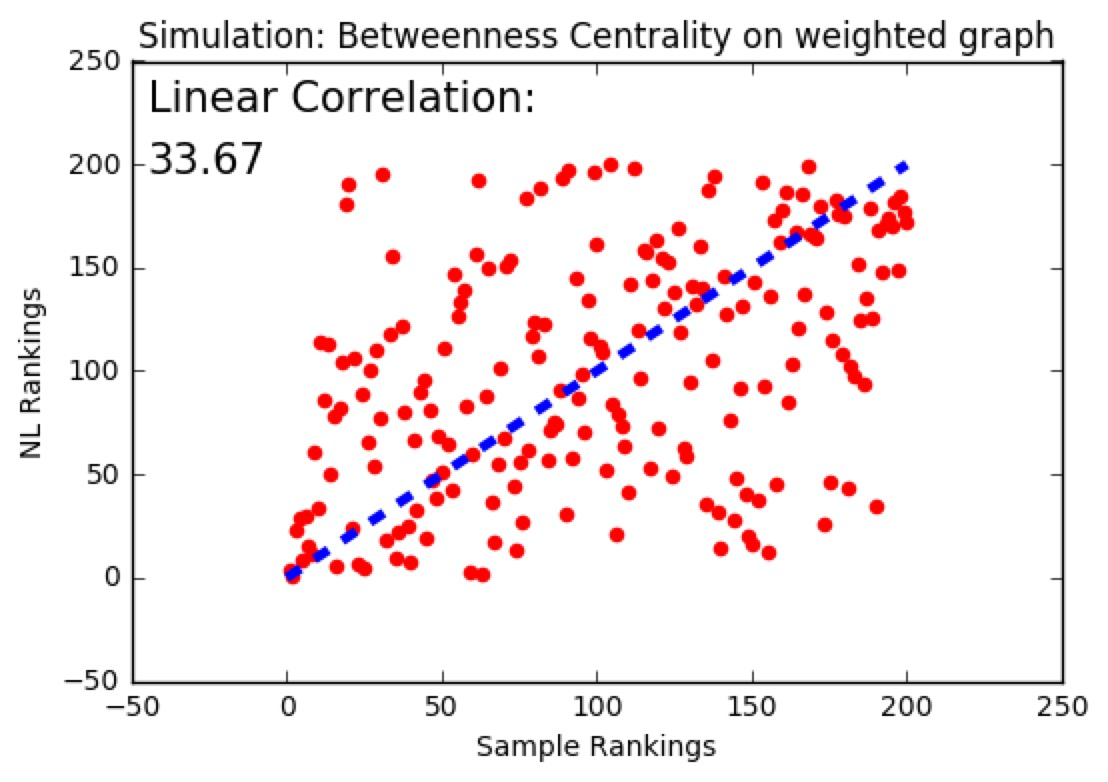
\includegraphics[width=0.95\linewidth]{BCW_NL.jpeg}
%  \caption{Per-map suboptimality}
%  \label{acpermap}
\end{subfigure}
%\caption{Normalized mean suboptimality on the per-map and uni-map bases for GBDT, SVM, and NN classifiers using AlexNet as a feature extractor}
\begin{subfigure}{.32\textwidth}
	\centering
    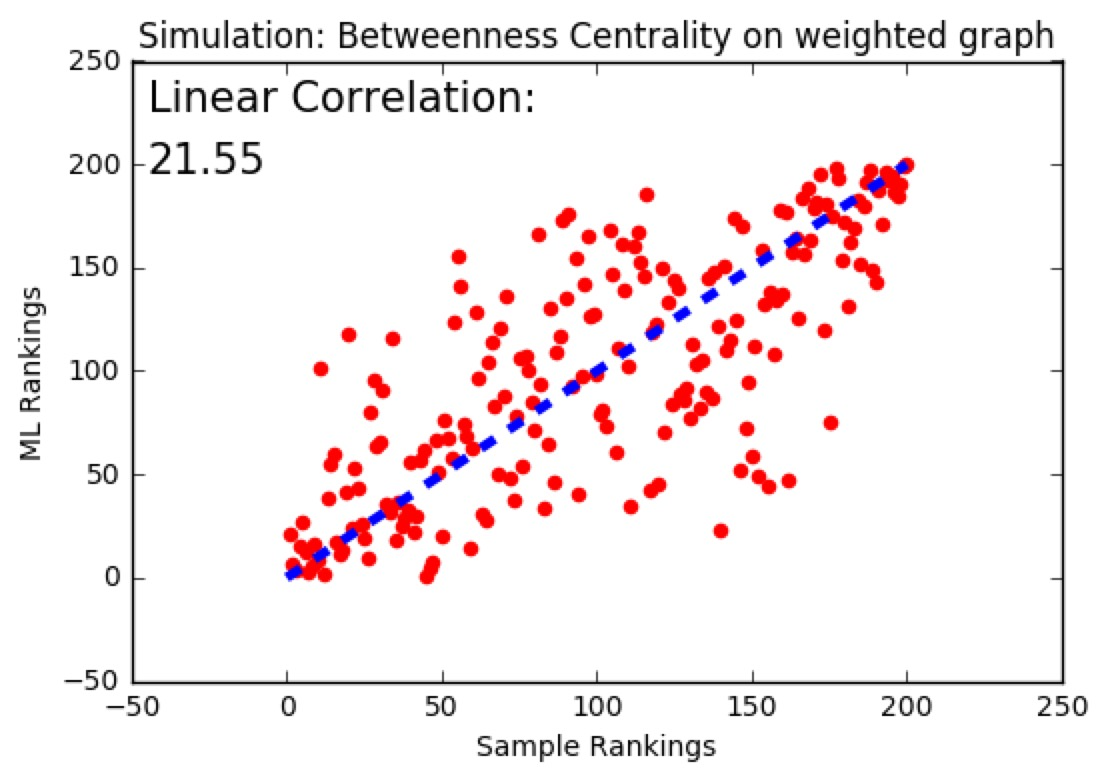
\includegraphics[width=0.95\linewidth]{BCW_ML.jpeg}
\end{subfigure}
%\label{alexclass}
\begin{subfigure}{.32\textwidth}
	\centering
    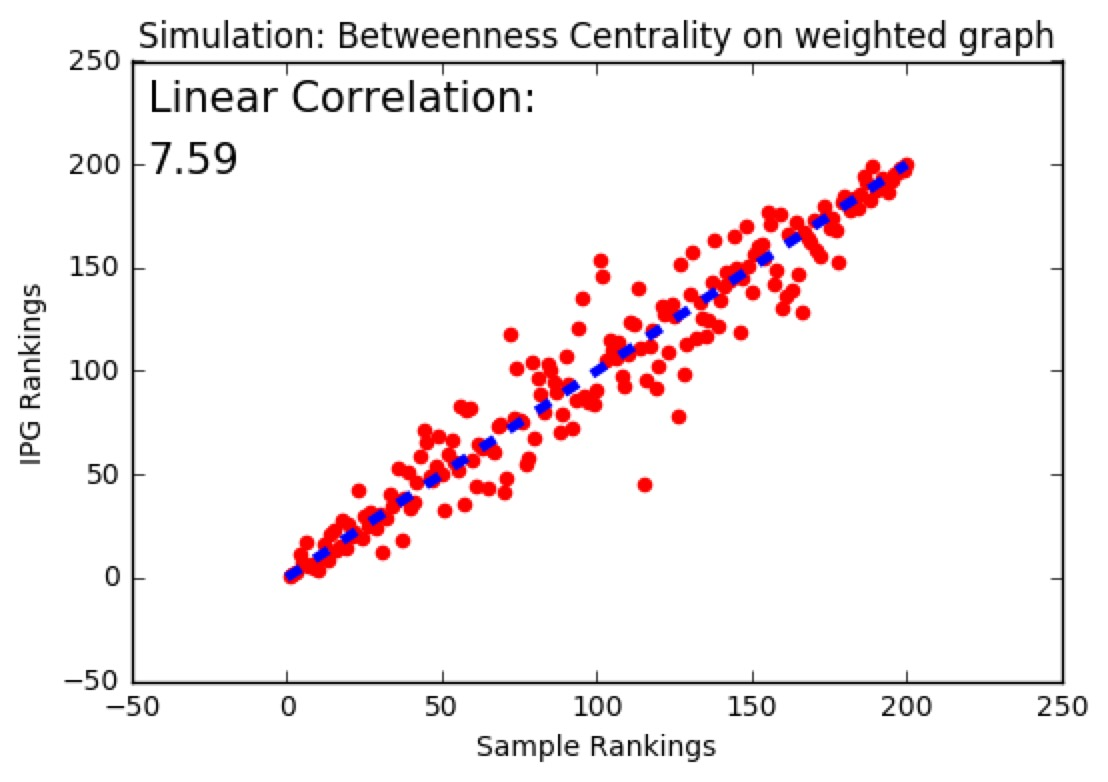
\includegraphics[width=0.95\linewidth]{BCW_IPG.jpeg}
\end{subfigure}
\caption{Comparison of betweenness centralities computed by different methods on simulated weighted graphs}
\end{figure}
\vspace{-0.1in}
\begin{figure}[H]
\centering
\begin{subfigure}{.32\textwidth}
  \centering
  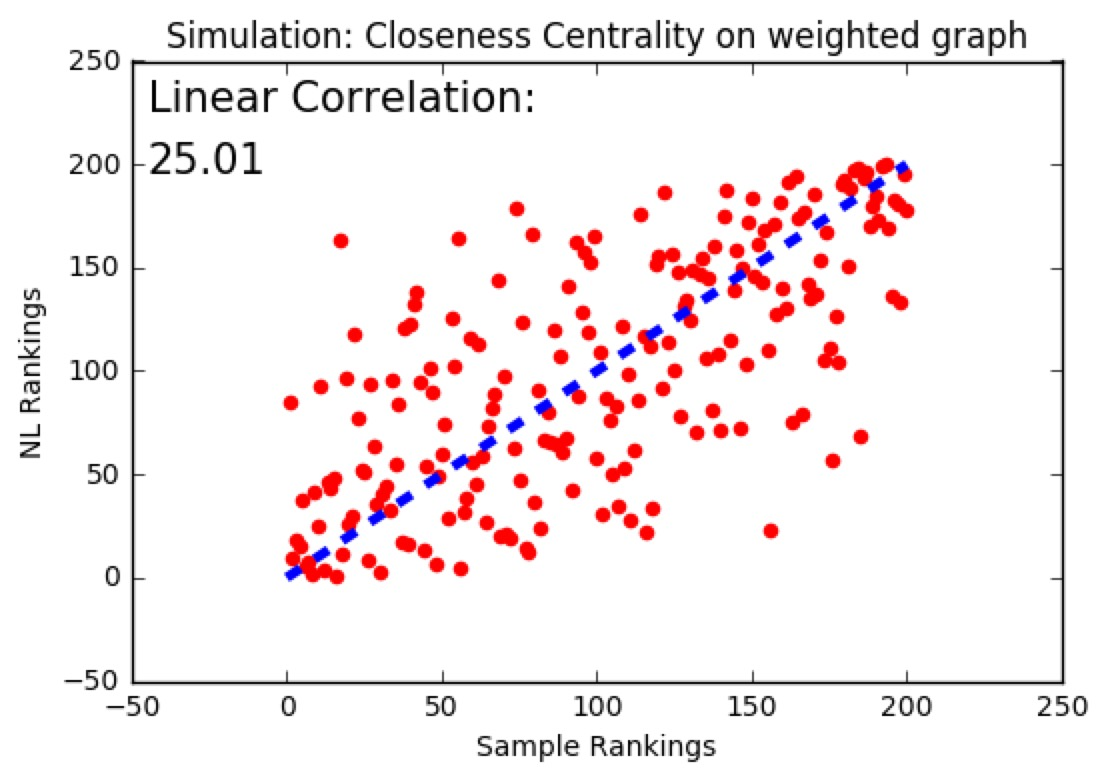
\includegraphics[width=0.95\linewidth]{CCW_NL.jpeg}
%  \caption{Per-map suboptimality}
%  \label{acpermap}
\end{subfigure}
%\caption{Normalized mean suboptimality on the per-map and uni-map bases for GBDT, SVM, and NN classifiers using AlexNet as a feature extractor}
\begin{subfigure}{.32\textwidth}
	\centering
    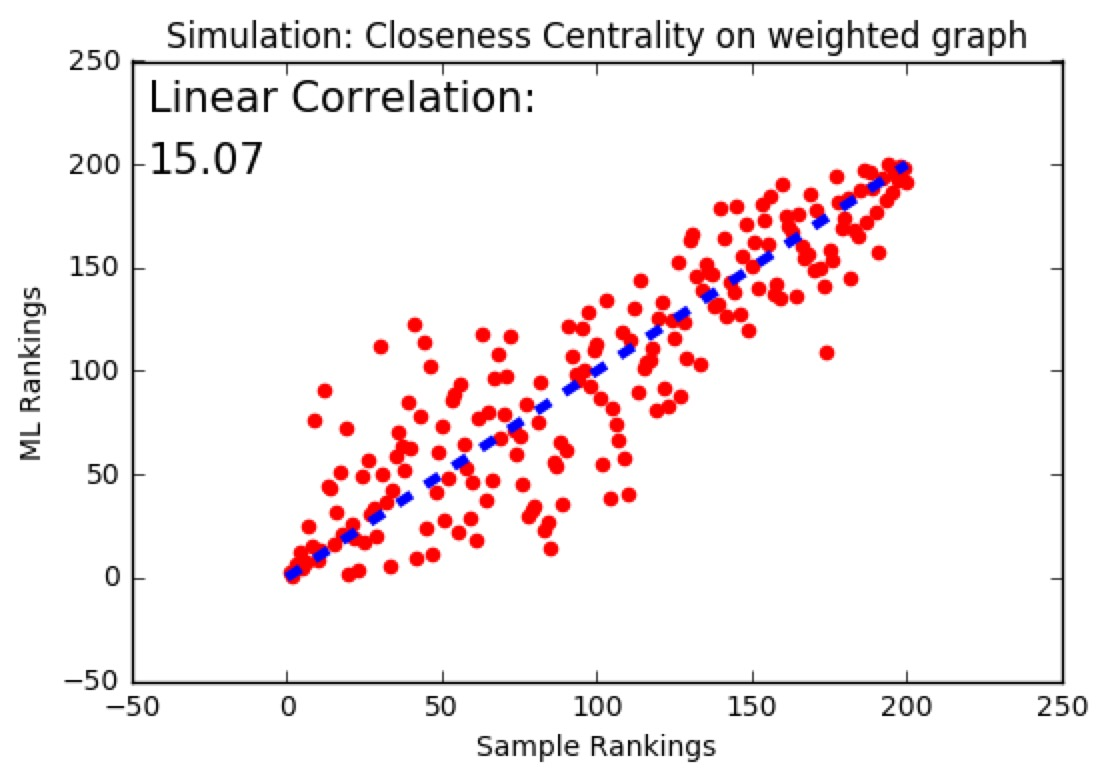
\includegraphics[width=0.95\linewidth]{CCW_ML.jpeg}
\end{subfigure}
%\label{alexclass}
\begin{subfigure}{.32\textwidth}
	\centering
    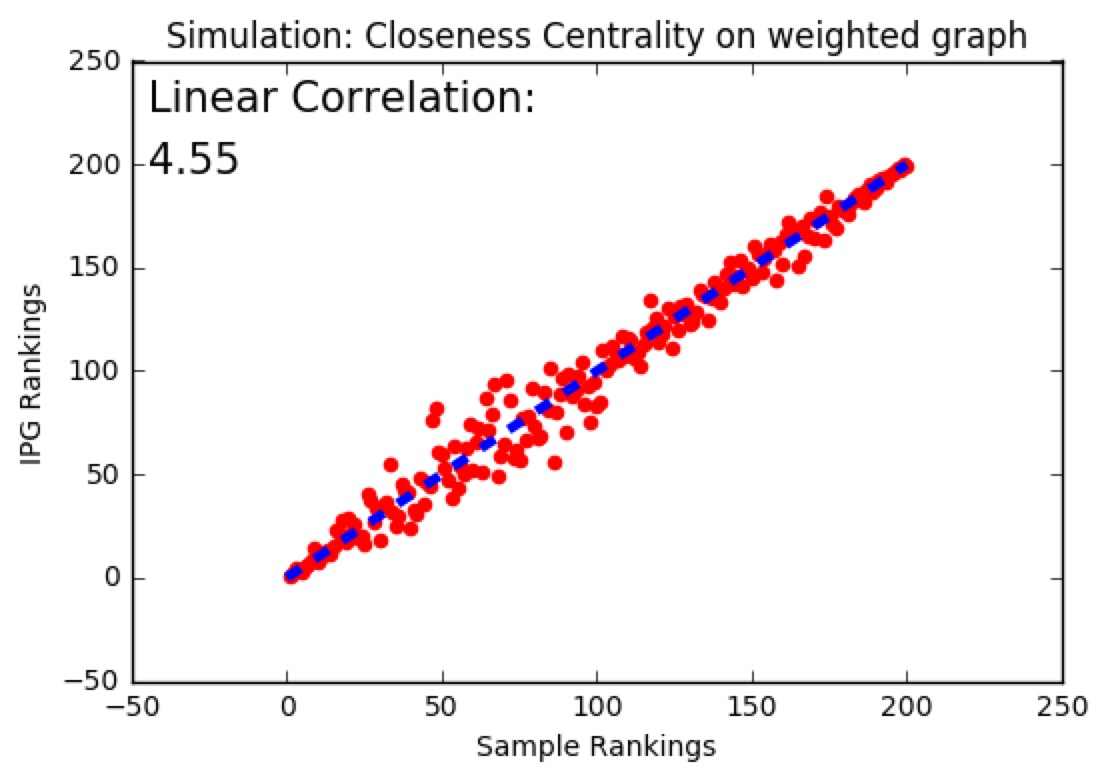
\includegraphics[width=0.95\linewidth]{CCW_IPG.jpeg}
\end{subfigure}
\caption{Comparison of closeness centralities computed by different methods on simulated weighted graphs}
\end{figure}
%\caption{Betweenness Centrality on Enron Dataset}
\end{frame}


\begin{frame}
\frametitle{Selection of Optimal Hyper-parameter $\lambda$}
\vspace{0.15in}
\begin{figure}[H]
\centering
\begin{subfigure}{.4\textwidth}
  \centering
  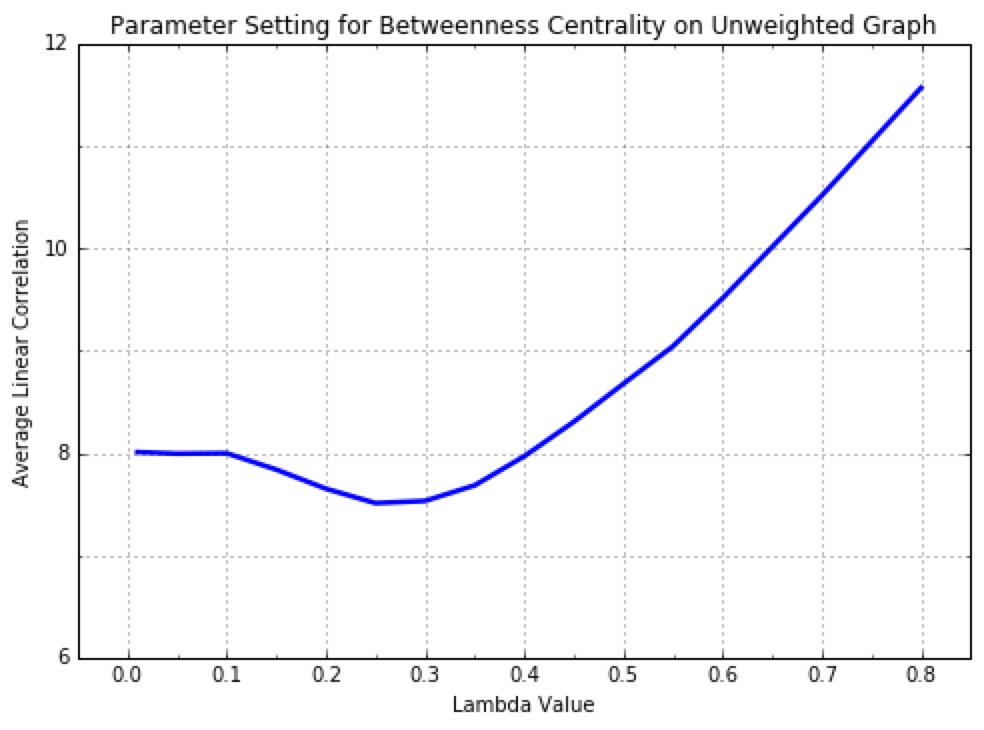
\includegraphics[width=0.95\linewidth]{BCU_2.jpeg}
%  \caption{Per-map suboptimality}
%  \label{acpermap}
\end{subfigure}
%\caption{Normalized mean suboptimality on the per-map and uni-map bases for GBDT, SVM, and NN classifiers using AlexNet as a feature extractor}
\begin{subfigure}{.4\textwidth}
	\centering
    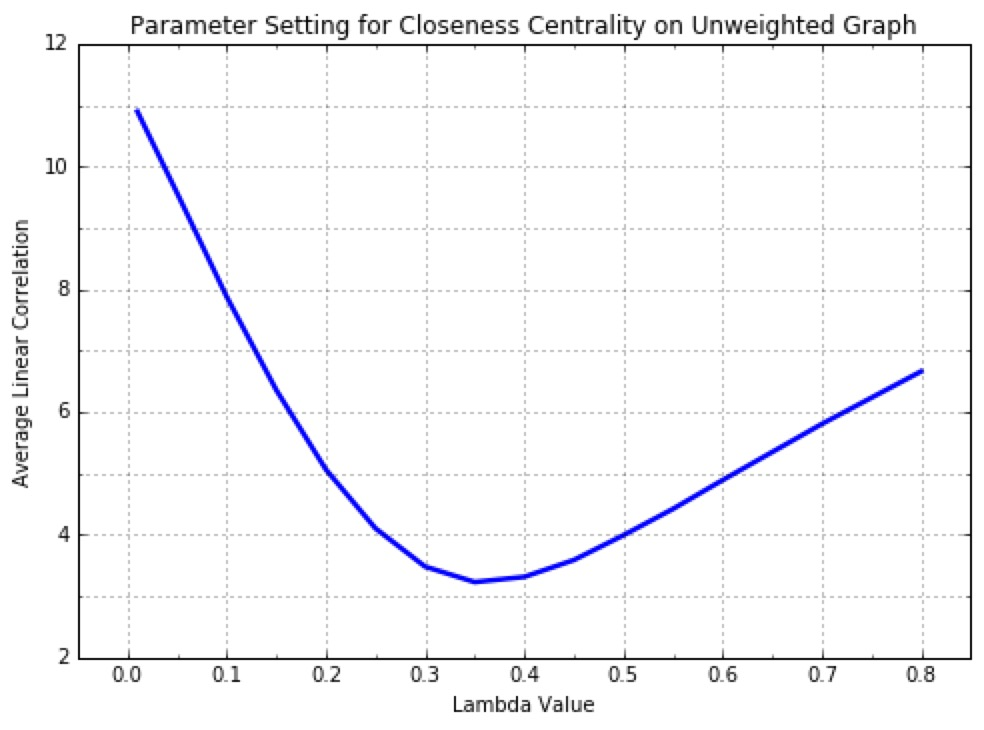
\includegraphics[width=0.95\linewidth]{CCU_2.jpeg}
\end{subfigure}

%\caption{Comparison of betweenness centralities computed by different methods on simulated weighted graphs}

\vspace{-0.1in}

\centering
\begin{subfigure}{.4\textwidth}
  \centering
  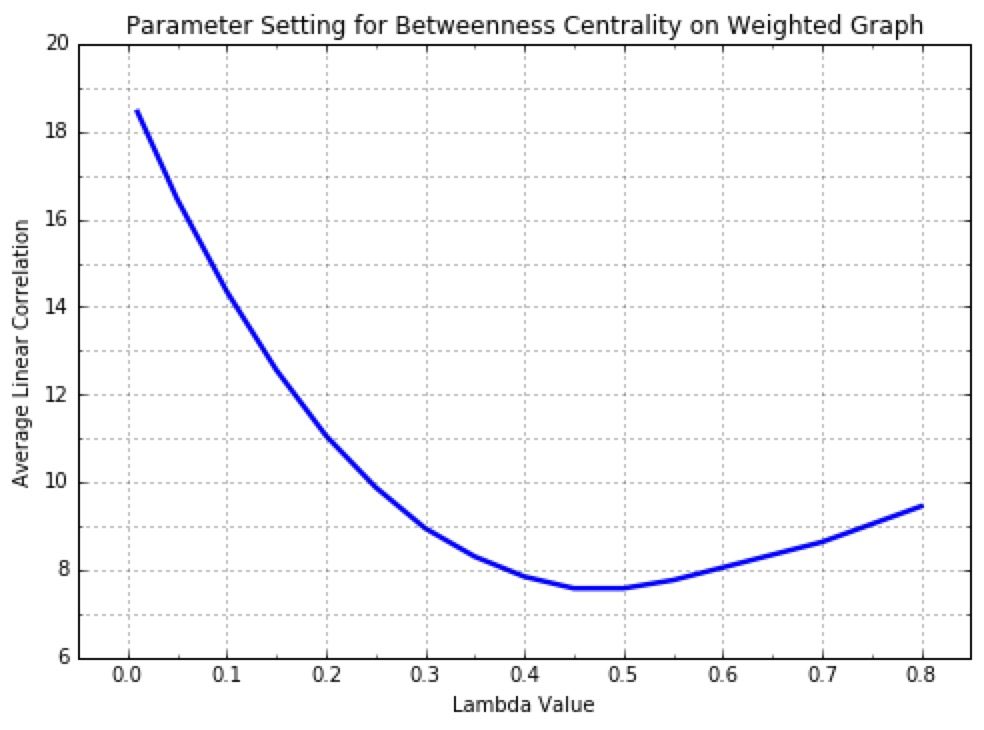
\includegraphics[width=0.95\linewidth]{BCW_2.jpeg}
%  \caption{Per-map suboptimality}
%  \label{acpermap}
\end{subfigure}
%\caption{Normalized mean suboptimality on the per-map and uni-map bases for GBDT, SVM, and NN classifiers using AlexNet as a feature extractor}
\begin{subfigure}{.4\textwidth}
	\centering
    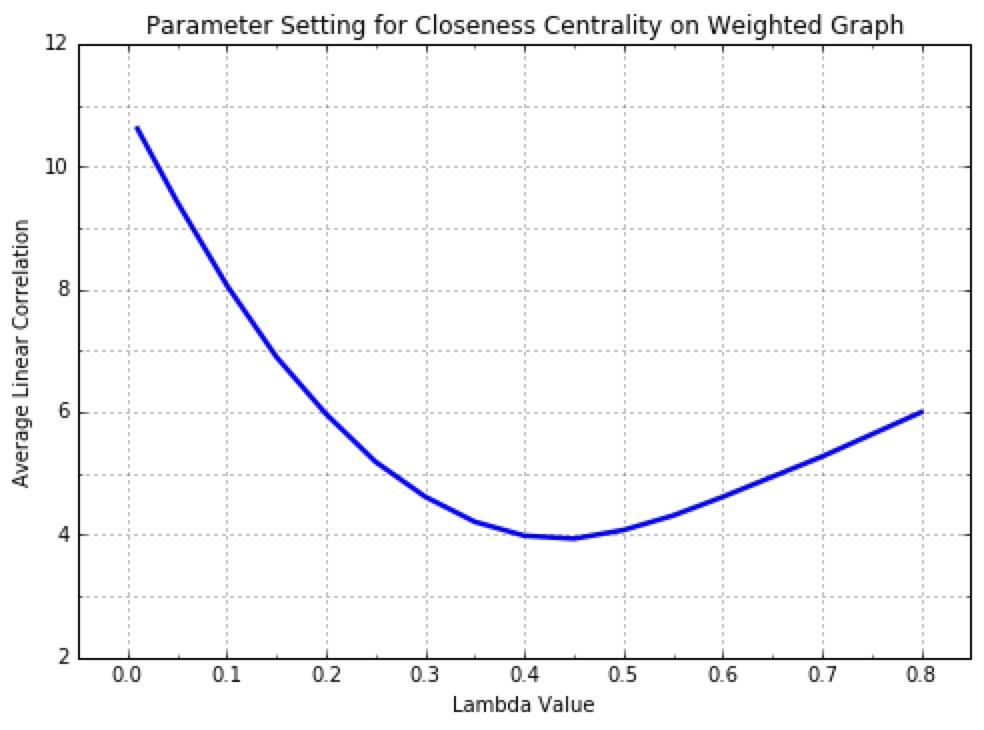
\includegraphics[width=0.95\linewidth]{CCW_2.jpeg}
\end{subfigure}
\caption{Hyper-parameter validation}
\end{figure}
%\caption{Betweenness Centrality on Enron Dataset}
\end{frame}



\section{Summary and Future Direction}
\begin{frame}
\frametitle{Summary}
\begin{itemize}
\item In this project we investigated the problem of calculating shortest path and centralities in the presence of edge uncertainty
\item We demonstrated the inability of taking the negative logarithm of edge probability as new edge weight
\item Based on the method of \textit{Most Probable Path}, we proposed a new and more direct way of computing shortest path and centralities of a graph, \textbf{Inversed Probabilistic Graph}
\item We empirically showed that under multiple circumstances, our approach outperforms previous approaches on related applications
\end{itemize}
\end{frame}

\begin{frame}
\frametitle{Future Direction}
Future directions can include research on
\begin{itemize}
\item How to detect community in the presence of edge uncertainty.
\end{itemize}
\end{frame}



%%%%%%%%%%%%%%%%%%%%%%%%%%%%%%%%%%%%%%%%%%%%%%%%%%%%%%%%%%%%%%%%%

% \begin{frame}{Font feature test}
%   \begin{itemize}
%     \item Regular
%     \item \textit{Italic}
%     \item \textsc{SmallCaps}
%     \item \textbf{Bold}
%     \item \textbf{\textit{Bold Italic}}
%     \item \textbf{\textsc{Bold SmallCaps}}
%     \item \texttt{Monospace}
%     \item \texttt{\textit{Monospace Italic}}
%     \item \texttt{\textbf{Monospace Bold}}
%     \item \texttt{\textbf{\textit{Monospace Bold Italic}}}
%   \end{itemize}
% \end{frame}

% \begin{frame}{Lists}
%   \begin{columns}[T,onlytextwidth]
%     \column{0.33\textwidth}
%       Items
%       \begin{itemize}
%         \item Milk \item Eggs \item Potatos
%       \end{itemize}

%     \column{0.33\textwidth}
%       Enumerations
%       \begin{enumerate}
%         \item First, \item Second and \item Last.
%       \end{enumerate}

%     \column{0.33\textwidth}
%       Descriptions
%       \begin{description}
%         \item[PowerPoint] Meeh. \item[Beamer] Yeeeha.
%       \end{description}
%   \end{columns}
% \end{frame}
% \begin{frame}{Animation}
%   \begin{itemize}[<+- | alert@+>]
%     \item \alert<4>{This is\only<4>{ really} important}
%     \item Now this
%     \item And now this
%   \end{itemize}
% \end{frame}
% \begin{frame}{Figures}
%   \begin{figure}
%     \newcounter{density}
%     \setcounter{density}{20}
%     \begin{tikzpicture}
%       \def\couleur{alerted text.fg}
%       \path[coordinate] (0,0)  coordinate(A)
%                   ++( 90:5cm) coordinate(B)
%                   ++(0:5cm) coordinate(C)
%                   ++(-90:5cm) coordinate(D);
%       \draw[fill=\couleur!\thedensity] (A) -- (B) -- (C) --(D) -- cycle;
%       \foreach \x in {1,...,40}{%
%           \pgfmathsetcounter{density}{\thedensity+20}
%           \setcounter{density}{\thedensity}
%           \path[coordinate] coordinate(X) at (A){};
%           \path[coordinate] (A) -- (B) coordinate[pos=.10](A)
%                               -- (C) coordinate[pos=.10](B)
%                               -- (D) coordinate[pos=.10](C)
%                               -- (X) coordinate[pos=.10](D);
%           \draw[fill=\couleur!\thedensity] (A)--(B)--(C)-- (D) -- cycle;
%       }
%     \end{tikzpicture}
%     \caption{Rotated square from
%     \href{http://www.texample.net/tikz/examples/rotated-polygons/}{texample.net}.}
%   \end{figure}
% \end{frame}
% \begin{frame}{Tables}
%   \begin{table}
%     \caption{Largest cities in the world (source: Wikipedia)}
%     \begin{tabular}{lr}
%       \toprule
%       City & Population\\
%       \midrule
%       Mexico City & 20,116,842\\
%       Shanghai & 19,210,000\\
%       Peking & 15,796,450\\
%       Istanbul & 14,160,467\\
%       \bottomrule
%     \end{tabular}
%   \end{table}
% \end{frame}
% \begin{frame}{Blocks}
%   Three different block environments are pre-defined and may be styled with an
%   optional background color.

%   \begin{columns}[T,onlytextwidth]
%     \column{0.5\textwidth}
%       \begin{block}{Default}
%         Block content.
%       \end{block}

%       \begin{alertblock}{Alert}
%         Block content.
%       \end{alertblock}

%       \begin{exampleblock}{Example}
%         Block content.
%       \end{exampleblock}

%     \column{0.5\textwidth}

%       \metroset{block=fill}

%       \begin{block}{Default}
%         Block content.
%       \end{block}

%       \begin{alertblock}{Alert}
%         Block content.
%       \end{alertblock}

%       \begin{exampleblock}{Example}
%         Block content.
%       \end{exampleblock}

%   \end{columns}
% \end{frame}
% \begin{frame}{Math}
%   \begin{equation*}
%     e = \lim_{n\to \infty} \left(1 + \frac{1}{n}\right)^n
%   \end{equation*}
% \end{frame}
% \begin{frame}{Line plots}
%   \begin{figure}
%     \begin{tikzpicture}
%       \begin{axis}[
%         mlineplot,
%         width=0.9\textwidth,
%         height=6cm,
%       ]

%         \addplot {sin(deg(x))};
%         \addplot+[samples=100] {sin(deg(2*x))};

%       \end{axis}
%     \end{tikzpicture}
%   \end{figure}
% \end{frame}
% \begin{frame}{Bar charts}
%   \begin{figure}
%     \begin{tikzpicture}
%       \begin{axis}[
%         mbarplot,
%         xlabel={Foo},
%         ylabel={Bar},
%         width=0.9\textwidth,
%         height=6cm,
%       ]

%       \addplot plot coordinates {(1, 20) (2, 25) (3, 22.4) (4, 12.4)};
%       \addplot plot coordinates {(1, 18) (2, 24) (3, 23.5) (4, 13.2)};
%       \addplot plot coordinates {(1, 10) (2, 19) (3, 25) (4, 15.2)};

%       \legend{lorem, ipsum, dolor}

%       \end{axis}
%     \end{tikzpicture}
%   \end{figure}
% \end{frame}
% \begin{frame}{Quotes}
%   \begin{quote}
%     Veni, Vidi, Vici
%   \end{quote}
% \end{frame}

% {%
% \setbeamertemplate{frame footer}{My custom footer}
% \begin{frame}[fragile]{Frame footer}
%     \themename defines a custom beamer template to add a text to the footer. It can be set via
%     \begin{verbatim}\setbeamertemplate{frame footer}{My custom footer}\end{verbatim}
% \end{frame}
% }

\begin{frame}{References}
\bibliography{demo}
\bibliographystyle{unsrt}
\end{frame}



% \begin{frame}{Summary}

%   Get the source of this theme and the demo presentation from

%   \begin{center}\url{github.com/matze/mtheme}\end{center}

%   The theme \emph{itself} is licensed under a
%   \href{http://creativecommons.org/licenses/by-sa/4.0/}{Creative Commons
%   Attribution-ShareAlike 4.0 International License}.

%   \begin{center}\ccbysa\end{center}

% \end{frame}

\begin{frame}[standout]
  Questions?
\end{frame}

% \appendix

% \begin{frame}[fragile]{Backup slides}
%   Sometimes, it is useful to add slides at the end of your presentation to
%   refer to during audience questions.

%   The best way to do this is to include the \verb|appendixnumberbeamer|
%   package in your preamble and call \verb|\appendix| before your backup slides.

%   \themename will automatically turn off slide numbering and progress bars for
%   slides in the appendix.
% \end{frame}

% \begin{frame}[allowframebreaks]{References}

%   \bibliography{demo}
%   \bibliographystyle{abbrv}

% \end{frame}

\end{document}
